\chapter{Data Analysis}
\label{chap_ana}
\section{Analysis Overview}
\label{sec_4_overview}

The main aim of this analysis is to extract $J/\psi$ spectra at mid-rapidity region in p-Pb collisions.  
The analysis is performed using the data of p-Pb collisions at $\sqrt{s_{NN}} =$ 5.02 TeV collected during LHC Run1 in 2013.
$J/\psi$ decays into $e^{+}e^{-}$ pairs with the branching ratio $=$ 5.94 $\pm$ 0.06\% (c.f. $J/\psi\rightarrow\mu^{+}\mu^{-}$: 5.93\%)~\cite{bib_pdg}.
In the ALICE central barrel ($|\eta| <$ 0.9), electrons can be detected by mainly using the information of the ITS and the TPC. 
%As well as the minimum bias trigger, the TRD triggered data is also available for the dielectron analysis with at least one leg pt $>$ 2 GeV/c. 

The invariant cross section of $J/\psi$ production is calculated as following,  
\begin{equation}
  \frac{1}{2\pi p_{T}}\frac{d^{2}\sigma_{J/\psi}}{dp_{T}dy} =  \frac{1}{2\pi p_{T}}\frac{1}{BR(J/\psi\rightarrow e^{+}e^{-})} \times \frac{N_{J/\psi ,raw}}{\int{L}dt \times \epsilon \times \Delta y \Delta p_{T}}
\end{equation}
where $N_{J/\psi ,raw}$ is the number of reconstructed $J/\psi$ and $\epsilon$ is the detection efficiency of $J/\psi$. 
$\Delta p_{T}$ and $\Delta y$ are bin width of $p_{T}$ and y. 
$\int{L}dt$ is the integrated luminosity.

In p-Pb collisions, comparisons to pp results are crucial to understand nuclear matter effects. 
The cold nuclear matter effects are quantified by the nuclear modification factor ($R_{pPb}$),  
It is defined as, 
\begin{equation}
  R_{pPb} = \frac{Y_{pPb}}{\langle N_{coll}\rangle Y_{pp}}
\end{equation}
where $\langle N_{coll}\rangle$ is the average number of binary nucleus-nucleus collisions in p-Pb collisions and $Y_{pPb}$ and $Y_{pp}$ are the yields in p-Pb and pp collisions, respectively.
If there is no effects of nuclei, this value should be unity. 
%On the other hand, if the modification is observed in $R_{pPb}$, it can be admitted nuclear matter effects have to be considered. 
On the other hand, the deviation from unity indicates the presence of cold nuclear matter effects.
%In order to calculate the $R_{pPb}$, the invariant cross section of J$\psi$ has to be extracted. 

$R_{pPb}$ is calculated with the following equation in this analysis, 
\begin{equation}
  R_{pPb} (p_{T}) = \frac{ \frac{ dY_{J/\psi , pPb} }{ dp_{T}dy } }{<T_{pPb}>\times \frac{\sigma_{J/\psi, pp}}{dp_{T}dy}}
\end{equation}
where, $Y_{J/\psi , pPb}$ is the invariant yield of $J/\psi$ in p-Pb collisions. 
$T_{pPb}$ is called "Nuclear Thickness Function'' expressed as, 
\begin{equation}
  T_{pA}(b) = \int{dz \rho_{A}(b,z)} = \frac{\langle N_{coll}\rangle }{\sigma_{pp}}
\end{equation}
 where, b is the impact parameter of p-Pb collisions and $\rho_{A}(b, z)$ is the nuclear density with mass number A.  
It is simply understood as the number of nucleons in the region where incident proton pass through a nuclei. 
It is normalized to satisfy $\int{T_{pA}} =$ A.
In this case, $\langle T_{pPb}\rangle =$ 0.0983 $\pm$ 0.0035 $\rm{mb}^{-1}$ is given by the Glauber model~\cite{bib_tppb}.
The uncertainties of $\sigma_{pPb}$ and $\langle N_{coll}\rangle$ can be canceled partialy by calculating ${T_{pA}}$.

For the extraction of the cross section, the procedure is following. 
After event selection from the recorded data, electrons are reconstructed using information of hits in ITS and TPC. 
Clean electron samples can be selected via information on their deposited energy in TPC. 
The next step is the calculation of invariant mass of $e^{+}e^{-}$ pairs. 
The invariant mass is calculated with the following equation, 
\begin{equation}
  m_{ee} = \sqrt{(E_{e^{+}}+E_{e^{-}})^{2}-(\vec{p_{e^{+}}} + \vec{p_{e^{-}}})^{2}}
\end{equation}
where $E_{e^{+}}$ and $E_{e^{+}}$ are energy and $\vec{p_{e^{+}}}$ and $\vec{p_{e^{-}}}$ are momentum of electrons and positrons, respectively.
J/$\psi$ signals are identified as a clear peak around $J/\psi$ mass (3.096 GeV/$c^{2}$)~\cite{bib_pdg}. 
To extract the number of reconstructed J/$\psi$ signals, background subtraction is needed. 
The main source of the background is combinatorial pairs from different decay processes. 
In order to evaluate the combinatorial pairs, the event mixing technique is adopted.  
After the raw signal extraction, acceptance and efficiency correction is done to calculate the invariant spectra of $J/\psi$.

pp reference spectra for $R_{pPb}$ are extracted by interpolating from measured pp spectra at different collision energies since there is no measurements in pp at $\sqrt{s_{NN}} = $ 5.02 TeV. 

In this chapter, the event selection is discussed first in Section.~\ref{sec_4_eventselection}.
Section~\ref{sec_4_trackrec} and \ref{sec_4_eid} describes how to reconstruct and select electron samples.  
Raw signal extraction of $J/\psi$ is discussed in Section.~\ref{sec_4_signalextraction}. 
Acceptance and efficiency correction is explained in Section.\ref{sec_4_correction}. 
%And then, the extraction of invariant yield is shown in this section.
The extraction of pp reference is also discussed in Section.~\ref{sec_4_ppref}.
%The calculation of the scaling factor is described in Section.\ref{sec_4_thickfunc}

\section{Event Selection}
\label{sec_4_eventselection}
\subsection{Minimum Bias Event Selection}
Minimum bias events are triggered using information of V0, T0 and SPD in 800 ns after a collision. 
In this analysis, the criteria of the minimum bias trigger is coincidence of both hits in V0A and V0C.
%\begin{itemize}
% \item Signal hit on the VZERO-A detector
% \item Signal hit on the VZERO-C detector
%\end{itemize}
In this condition, the trigger efficiency of the minimum bias events is 96.4\%. 
To reduce fake events caused by beam-gas and beam-halo collisions, the timing information of VZERO and TZERO are used. 

%should be discussed about pile-up?
%The $\mu$ of pile-up events for MB is about .
%Pile-up events are found by the primary vertex reconstruction using SPD. 
%The events which has at least 2 candidates of the primary vertex and fulfill the following requirements are rejected. 
%Primary vertex which is thought as the collision vertex is reconstructed by the hit on SPD detectors.
%It is determined as the 3-D center points of selected tracks by straight fitting and calculating the minimum closest point for the all track pairs,
%Primary vertex which is thought as the collision vertex is reconstructed by the hit on SPD detectors. 
%It is determined as the 3-D center points of selected tracks by straight fitting and calculating the minimum closest point for the all track pairs, 
Primary vertex is reconstructed as described in Section\ref{sec_3_vtx}. 
In this analysis, the minimum number of tracks which contribute to the determination of the primary vertex is required at least one tracks. 
\begin{itemize}
\item[-] $N_{contribute} >$ 1
\end{itemize}
Additionally, Z-position cut of the primary vertex is applied as following to keep the uniformity of the acceptance and reconstruction performance,  
Figure~\ref{fig_4_zvtx} shows the $Z_{vtx}$ distribution of the primary vertex in p-Pb collisions. 
\begin{itemize}
\item[-] $|Z_{vtx}| < $ 10 cm
\end{itemize} 
\begin{figure}[!h]
  \centering
  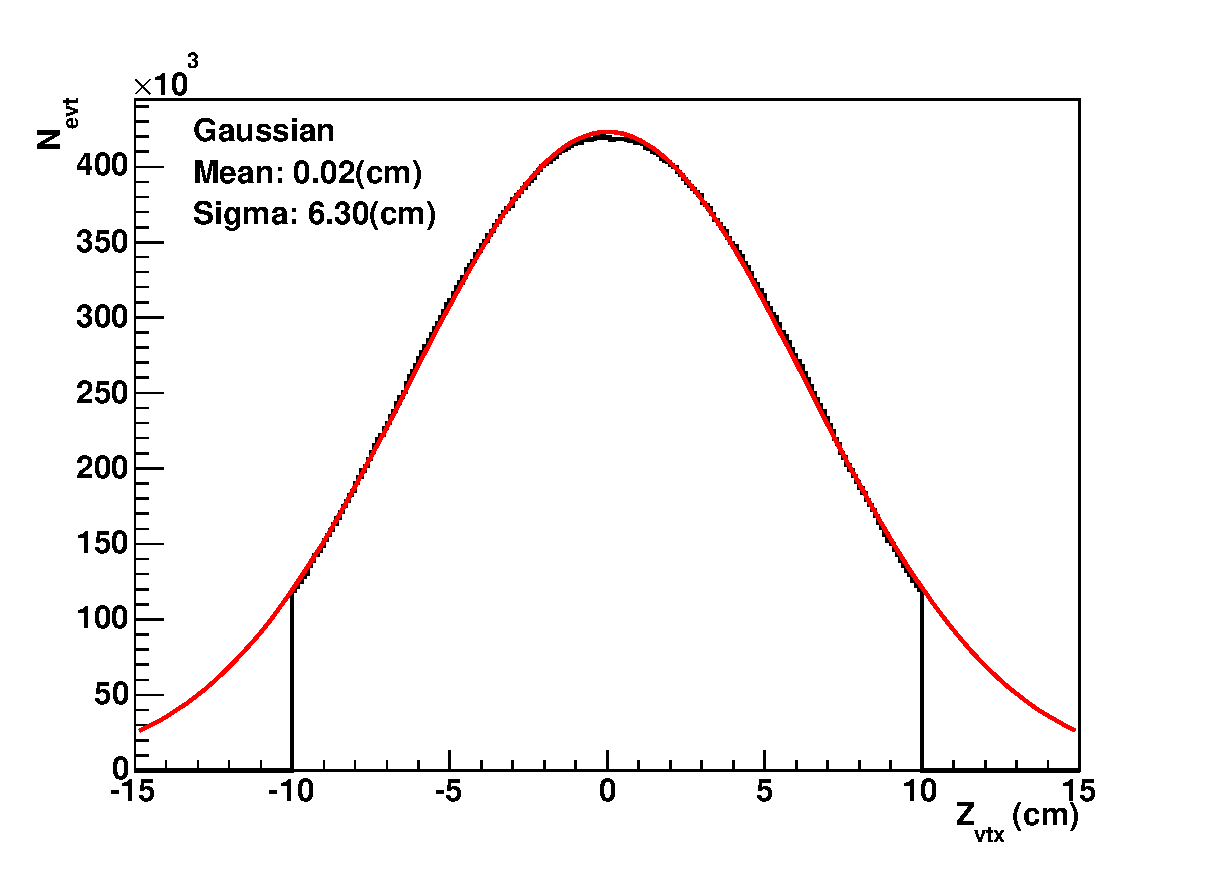
\includegraphics[width=10cm]{chap4/figure/QA/Zvtx_INT7.eps}
  \caption{$Z_{vtx}$ distribution of the accepted minimum bias events in p-Pb collisions.}
  \label{fig_4_zvtx}
\end{figure}

After the event selection, the number of selected events is 96 M events. 
The cross section of the minimum bias events triggered with V0 detector is 2.09 b $\pm$ 3.0\%  measured by van der Meer scan\cite{bib_v0cross}. 
Therefore the integrated luminosity is calculated as following, 
\begin{equation}
  \int{Ldt} = \frac{N_{MB,ana}}{\sigma_{V0}} = 96 M / 2.09 (b) = 48 \mu b^{-1}
\end{equation}

%\subsection{TRD Triggers Event Selection}
%The TRD trigger suffers from the secondary electrons from photon decays at large radii due to the straight line fit of track reconstruction as shown in Fig.~\ref{fig_4_fakeconv}. 
%\begin{figure}[!h]
%  \centering
%  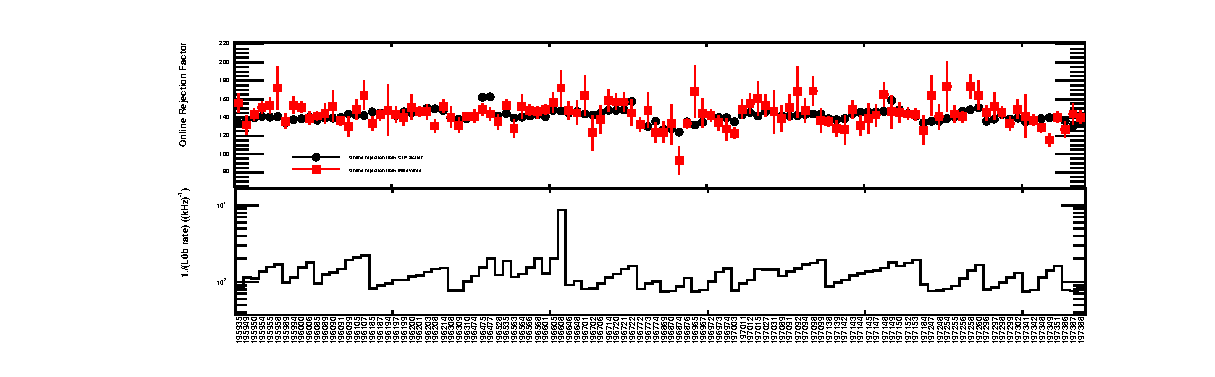
\includegraphics[width=18cm]{chap4/figure/TRDOnline/OnlineRejeandL0brate_LHC13ef.eps}
%  \caption{Run by run online event rejection factor during rare trigger runs in p-Pb collisions.}
%  \label{fig_4_}
%\end{figure}

%\begin{figure}[!h]
%  \centering
%  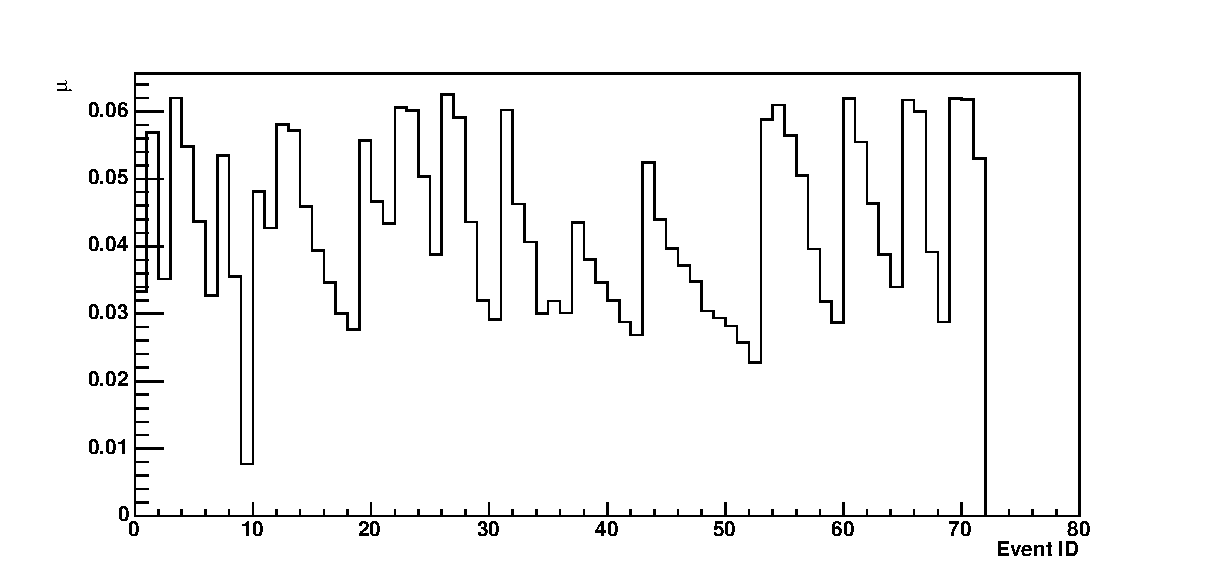
\includegraphics[width=15cm]{chap4/figure/TRDOnline/EventMu_LHC13f.eps}
%  \caption{Run by run $\mu$ of the poisson distribution.}
%  \label{fig_4_}
%\end{figure}
%\begin{figure}[!h]
%  \centering
%  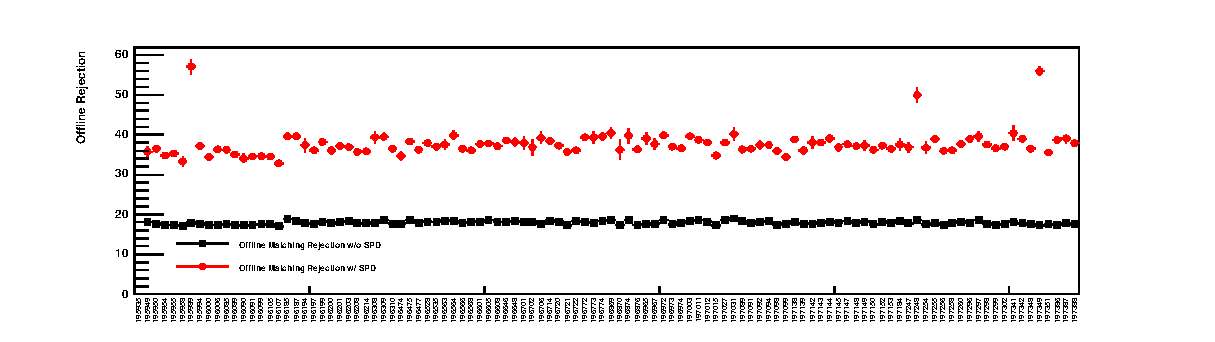
\includegraphics[width=15cm]{chap4/figure/TRDOnline/OfflineMatch_LHC13ef.eps}
%  \caption{Run by run online event rejection factor during rare trigger runs in p-Pb collisions.}
%  \label{fig_4_}
%\end{figure}
%\begin{figure}[!h]
%  \centering
%  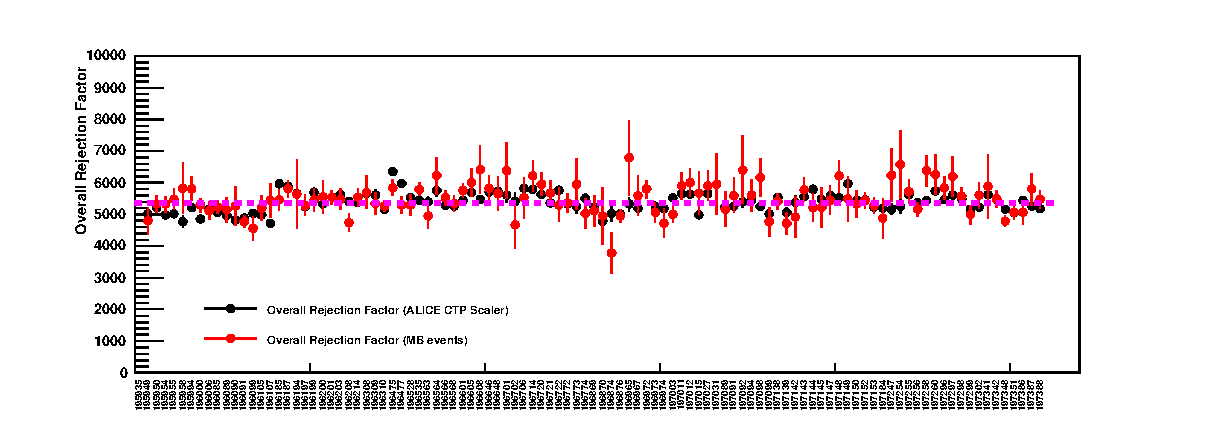
\includegraphics[width=15cm]{chap4/figure/TRDOnline/OverallRejection_LHC13ef.eps}
%  \caption{Run by run online event rejection factor during rare trigger runs in p-Pb collisions.}
%  \label{fig_4_}
%\end{figure}

%\begin{figure}[!h]
%  \centering
%  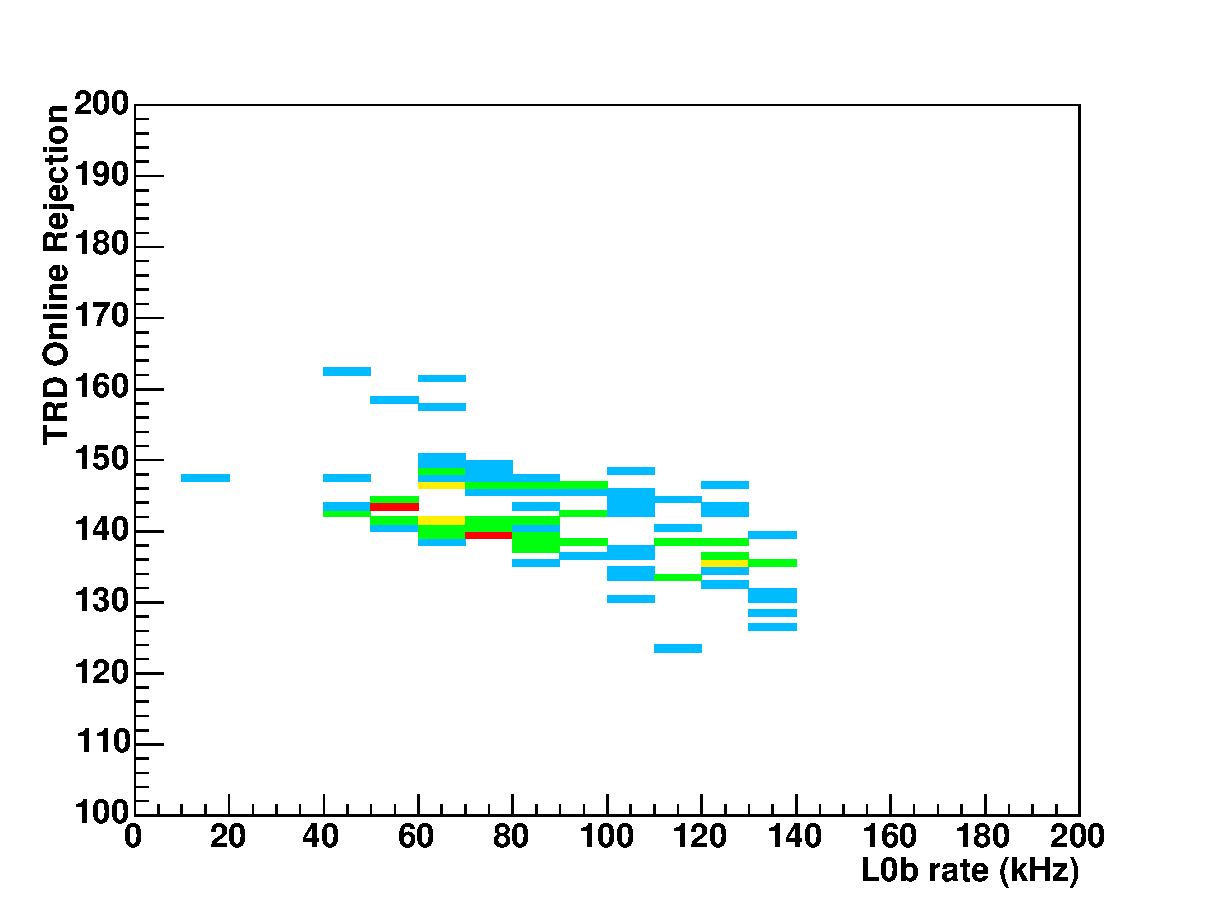
\includegraphics[width=9cm]{chap4/figure/TRDOnline/OnlineRejvsL0brate_log.eps}
%  \caption{Collision rate dependence on online rejection factor in p-Pb collisions}
%  \label{fig_4_}
%\end{figure}

%\begin{figure}[!h]
%  \centering
%  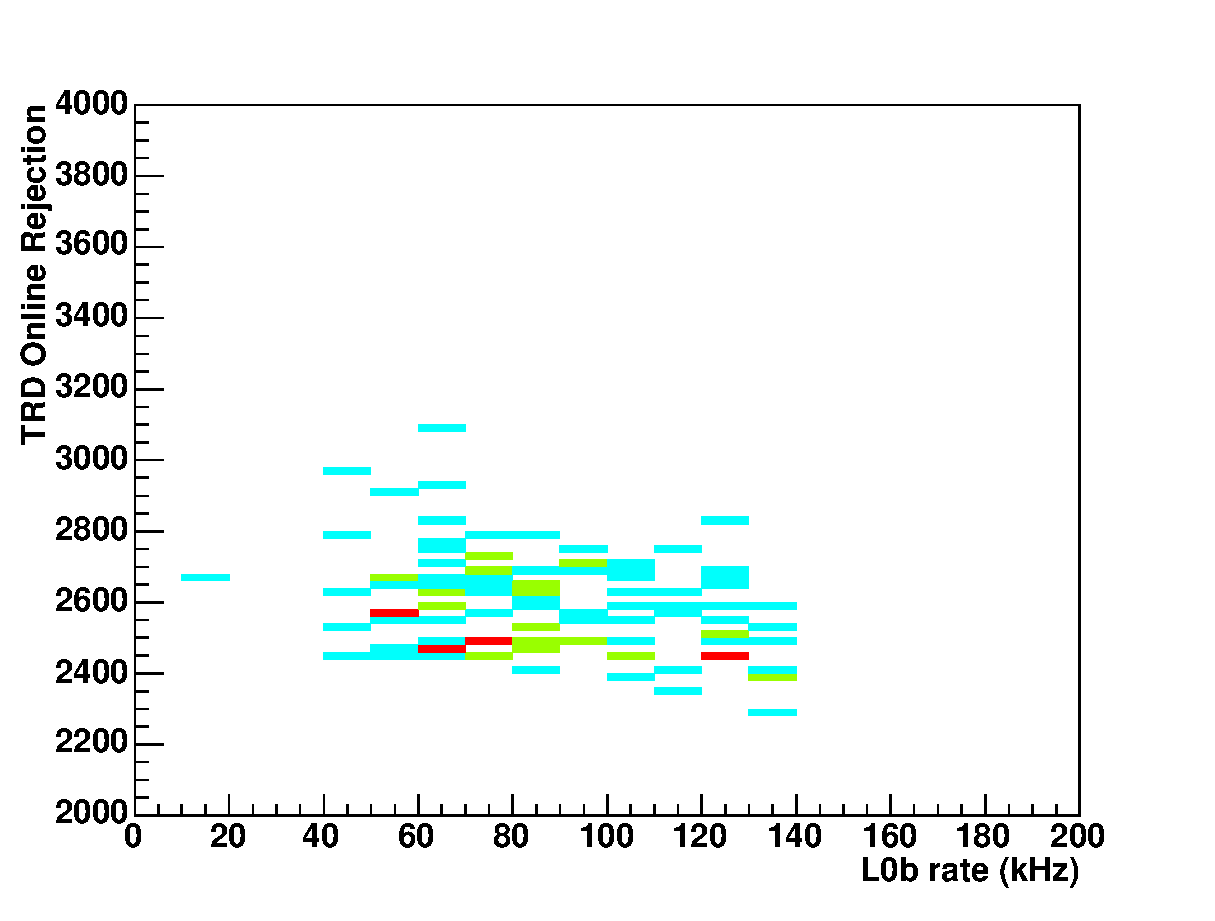
\includegraphics[width=9cm]{chap4/figure/TRDOnline/OnlineRejvsL0brateoff_log.eps}
%  \caption{Collision rate dependence on online rejection factor including offline matching in p-Pb collisions}
%  \label{fig_4_}
%\end{figure}

%\begin{figure}[!h]
%  \centering
%  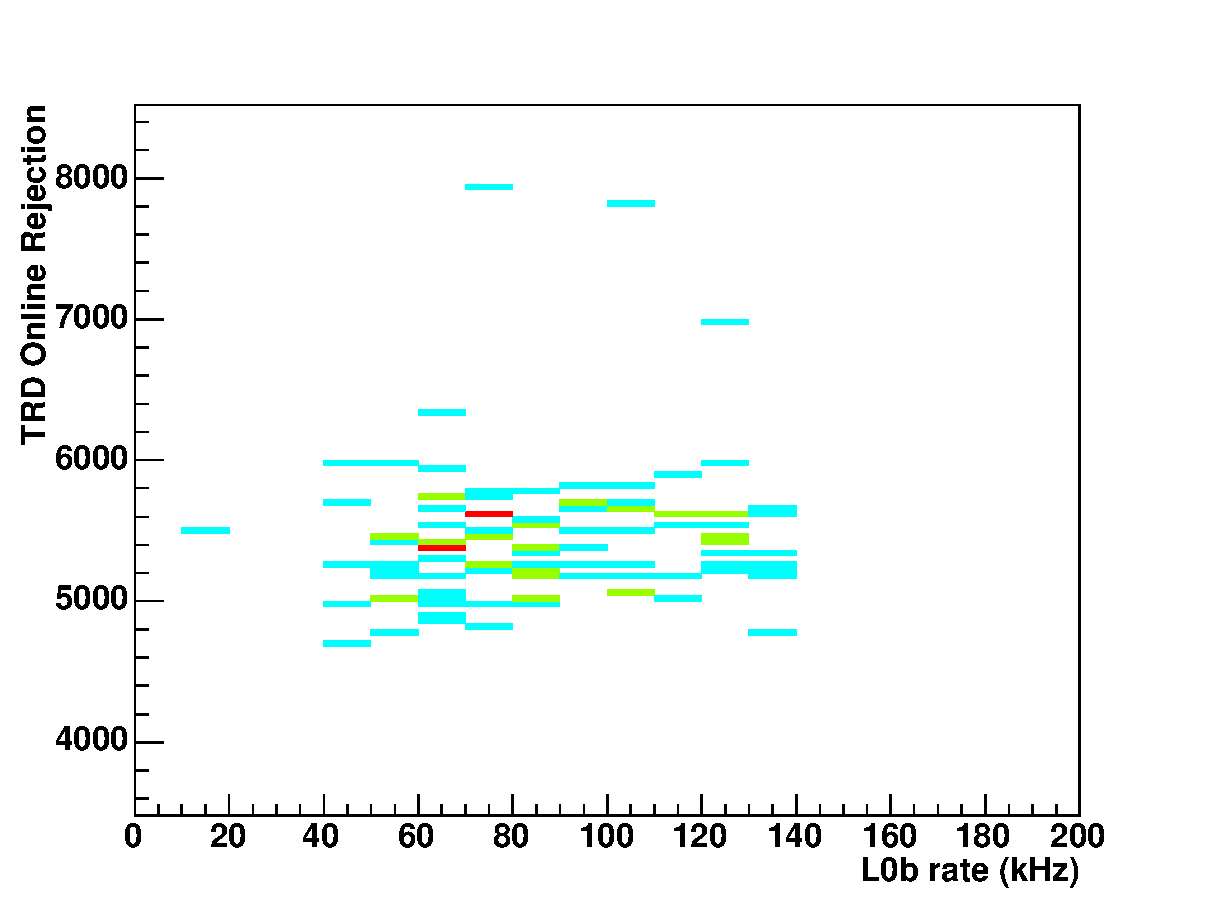
\includegraphics[width=9cm]{chap4/figure/TRDOnline/OnlineRejvsL0bratespd_log.eps}
%  \caption{Collision rate dependence on online rejection factor including SPD matching in p-Pb collisions}
%  \label{fig_4_}
%\end{figure}

%\begin{figure}[!h]
%  \centering
%  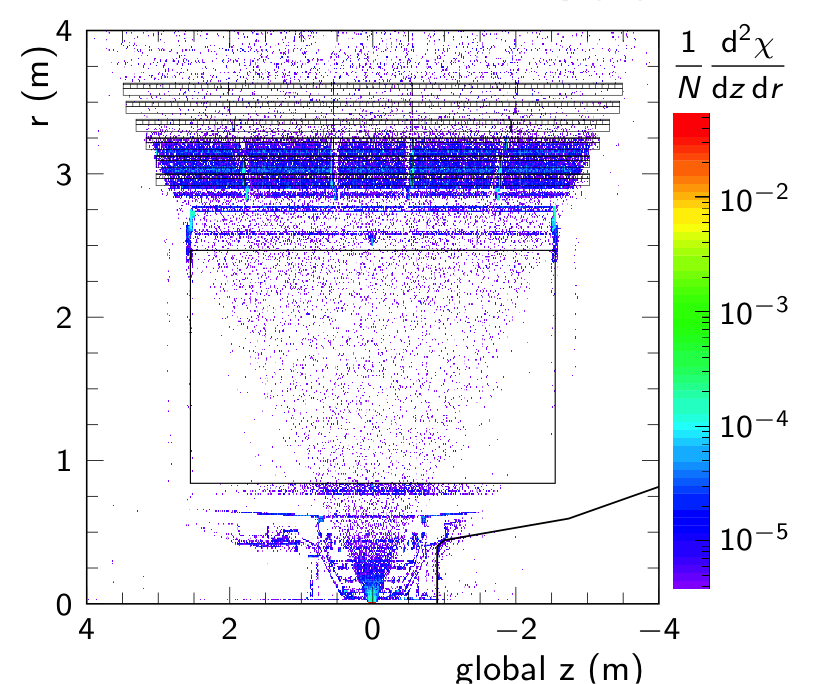
\includegraphics[width=10cm]{chap4/figure/TRDOnline/ConversionDisEta.png}
%  \caption{$\eta$ distribution of conversion electrons generated in the ALICE detectors.}
%  \label{fig_4_}
%\end{figure}

%\begin{figure}[!h]
%  \centering
%  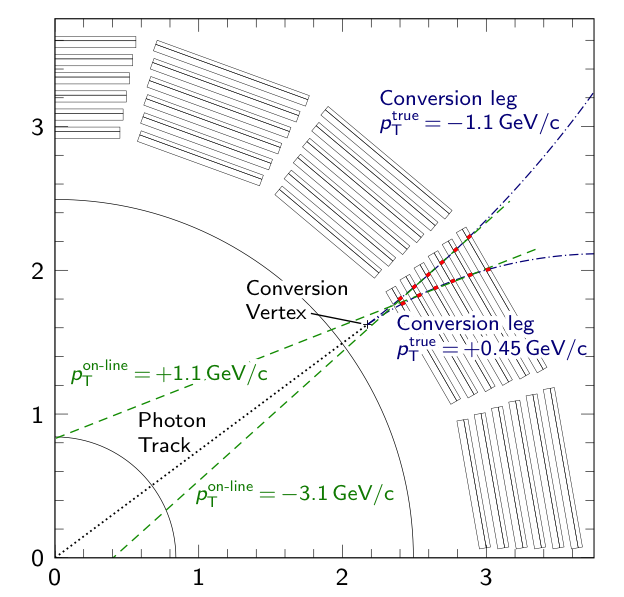
\includegraphics[width=10cm]{chap4/figure/TRDOnline/fake_conversion.png}
%  \caption{Example of fake trigger by late conversion electrons.}
%  \label{fig_4_fakeconv}
%\end{figure}
%The online rejection is determined by the pure TRD PID performance but the rate of conversion electrons. 
%In order to reduce the fake triggered events, the offline-online reconstructed track matching is required in the offline analysis. 
%Almost all fake fired electrons are produced at outer of TPC and then they are not reconstructed via ITS and TPC. 
%Figure shows the rejection of offline-online track matching ratio for each runs. 

%During TRD trigger runs, the interaction rate increased high up to 200 kHz and the out-of-bunch pileup tracks has to be taken into account because the drift time of TRD is 2 $\mu s$. 
%Figure\ref{fig_} shows the collision rate dependence of rejection factors of TRD. 
%The rejection factor become lower at high collision rate due to the out-of-bunch pileup.  
%To reduce the out-of-bunch pileup, the hit on the silicon pixel detector (SPD) is required. 
%SPD is the most inner detector of ITS. 
%The integration time of the SPD readout is 100 ns and it is enough short to reject the out-of-bunch tracks because the bunch crossing interval is 200 ns in p-Pb collisions. 

%The acceptance of TRD triggers for $J/\psi$


%\subsection{Event Characteristic Variables}
%In p-Pb collisions, it is very important to see the event activity dependence because the difference of event activity correspond to the different dynamics of collisions. 
%Multiplicity is determined in different rapidity windows. 
%At mid-rapidity ($\eta$ < 1) charge particle multiplicity is estimated using SPD tracklets defined as Section\ref{sec_3_ALICEcentral}. 
%The number of SPD tracklets is naively proportional to the charge particle multiplicity. 
%The top panels of Fig.~\ref{fig_4_spdtr_MB} show the raw SPD tracklets distribution as a function of $Z_vtx$. 
%SPD tracklets multiplicity depends on the acceptance of SPD and show the asymmetry of $Z_{vtx}$ distribution. 
%\begin{figure}[!h]
 % \centering
  %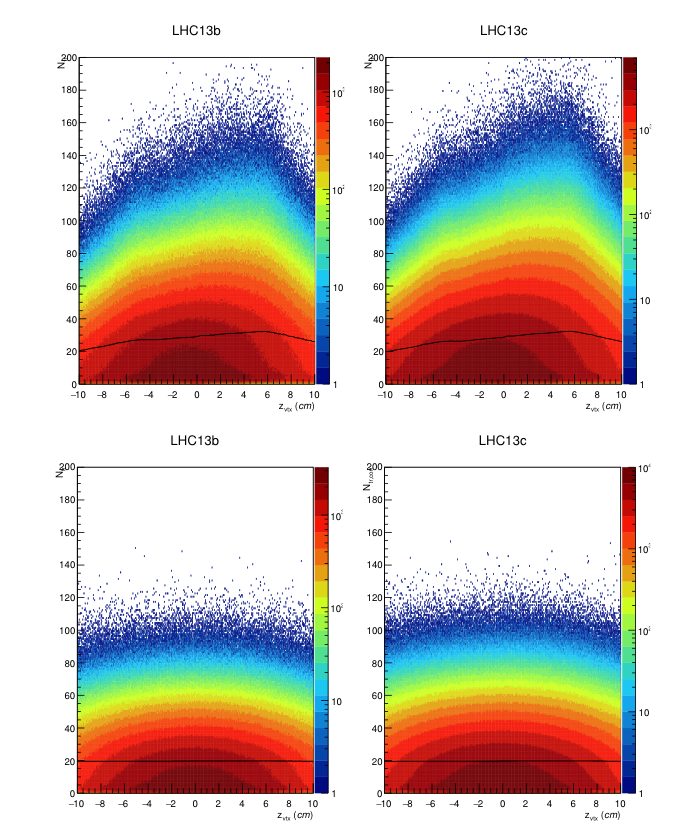
\includegraphics[width=15cm]{chap4/figure/EventActivity/SPDTracklets.png}
%  \caption{.}
%  \label{fig_4_spdtr_MB}
%\end{figure}

%In order to obtain good estimation of the charge particle multiplicity, a correction to uniform distribution for $Z_{vtx}$ is needed.
%The profile is used as an input ot renormalize $N_{tr}$ on an event-by-event-base from $<N_{tr}>$, which are 28.55 and 28.13 for LHC13b and LHC13c respectively, to the global minimum of the profile of LHC13c $<Ntr>_{glob}=$ 19.44.
%The correction factors are applied relating the global minimum to the local average $<N_{tr}>[Z_{vtx}]$ yielding from the profiles for LHC13b and LHC13c with a Poisson smearing, 
%\begin{equation}
%  \Delta_{N} = N_{tr}(\frac{<N_{tr}_{glob}>}{<N_{tr}>[z_{vtx}]}-1) 
%\end{equation}
%\begin{equation}
%  N^{corr}_{tr} = N_{tr} -Poisson(\Delta_{N})
%\end{equation}
%\begin{figure}[!h]
%  \centering
%  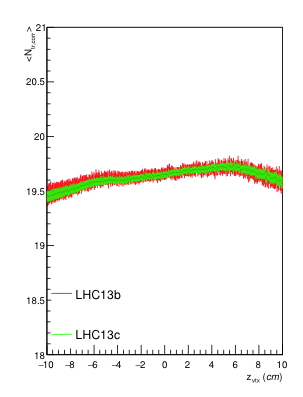
\includegraphics[width=8cm]{chap4/figure/EventActivity/MeanSPDTracklets.png}
%  \caption{.}
%  \label{fig_4_meanspdtr_MB}
%\end{figure}
%5The bottom panels of Fig.~\ref{fig_4_spdtr_MB} show the SPD tracklets multiplicity as a function of $Z_{vtx}$ after correction. 
%$<N_{tr}>$ become flat and uniform distribution is obtained in both run periods. %

%The same procedure is also done for V0A multiplicity as shown in Fig.~\ref{fig_v0atr_MB,fig_4_meanv0atr_MB}. 
%\begin{figure}[!h]
%  \centering
%  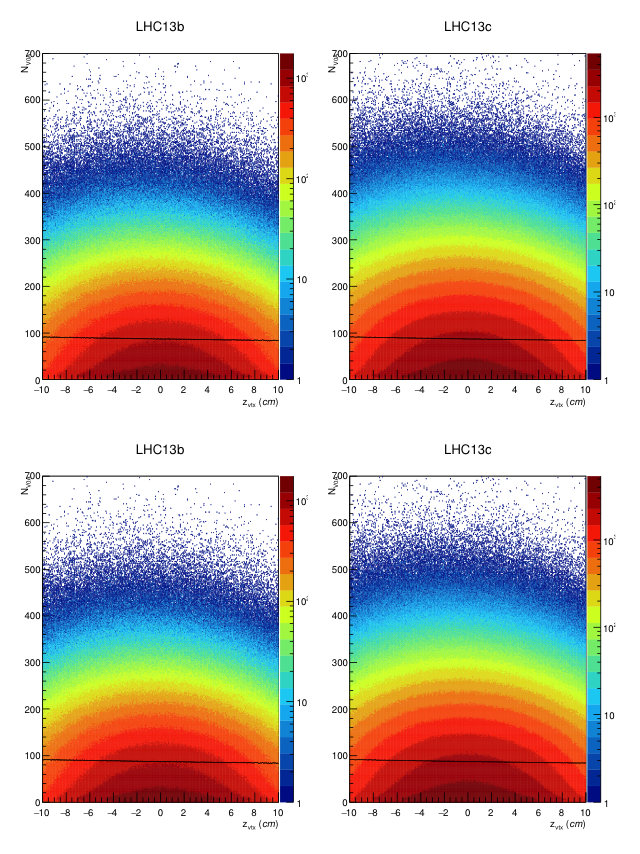
\includegraphics[width=15cm]{chap4/figure/EventActivity/V0ATracklets.png}
%  \caption{.}
%  \label{fig_4_v0atr_MB}
%\end{figure}

%\begin{figure}[!h]
%  \centering
%  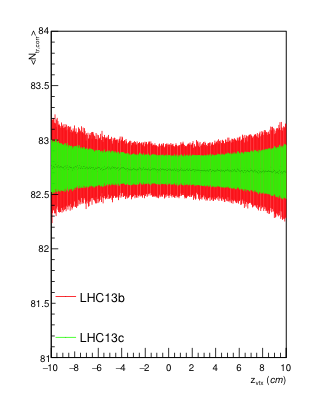
\includegraphics[width=8cm]{chap4/figure/EventActivity/MeanV0ATracklets.png}
%  \caption{.}
%  \label{fig_4_meanv0atr_MB}
%\end{figure}

%For the conversion of the corrected $N^{corr}_tr$ to $dN_{ch}/d\eta$ Monte-Carlo information is needed. 
%%In the dedicated MC samples we can count the number of charged particle tracks in .
%The $dN_{ch}/d\eta$ vs $N^{corr}_{tr}$ is plotted in Fig.\ref{fig_4_nchvsntr_MB}. 
%To obtain the linear dependence, a linear fit is done on the 2D distribution and each multiplicity intervals as shown in Fig.~\ref{fig_4_nchvsntr_MB} and $dN_{ch}/d\eta$ is calculated in each interval. 
%The relative deviation du to the perfect correction of $N^{corr}_{tr}$ is treated as a systematic uncertainty on the multiplicity variable.

%\begin{figure}[!h]
%  \centering
%  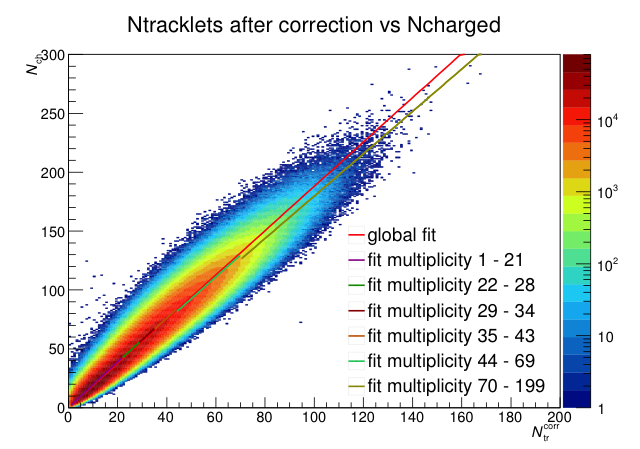
\includegraphics[width=10cm]{chap4/figure/EventActivity/NchvsNtr.png}
%  \caption{.}
%  \label{fig_4_nchvsntr_MB}
%\end{figure}


\section{Run Quality Check}
\label{sec_4_runselection}
For the stability of data, run quality check based on the number of electron candidates per event is performed. 
Before run-by-run quality assurance, 2 runs are already excluded due to the DAQ error and the check is done for 26 runs. 
Figure~\ref{fig_4_runqa_MB} shows the number of electron candidates after the electron identification divided by the number of analyzed events for each event in minimum bias run periods. 
Figure~\ref{fig_4_runqapro_MB} also shows the projection of the number of electron and positron sum per event for each run. 
The distribution can be described by gaussian well for all $p_{T}$ range and cut variation.
All runs are within 5 $\sigma$ from the mean points in all categories. 
Therefore all runs are enough stable and accepted.  

\begin{figure}[!h]
  \centering
  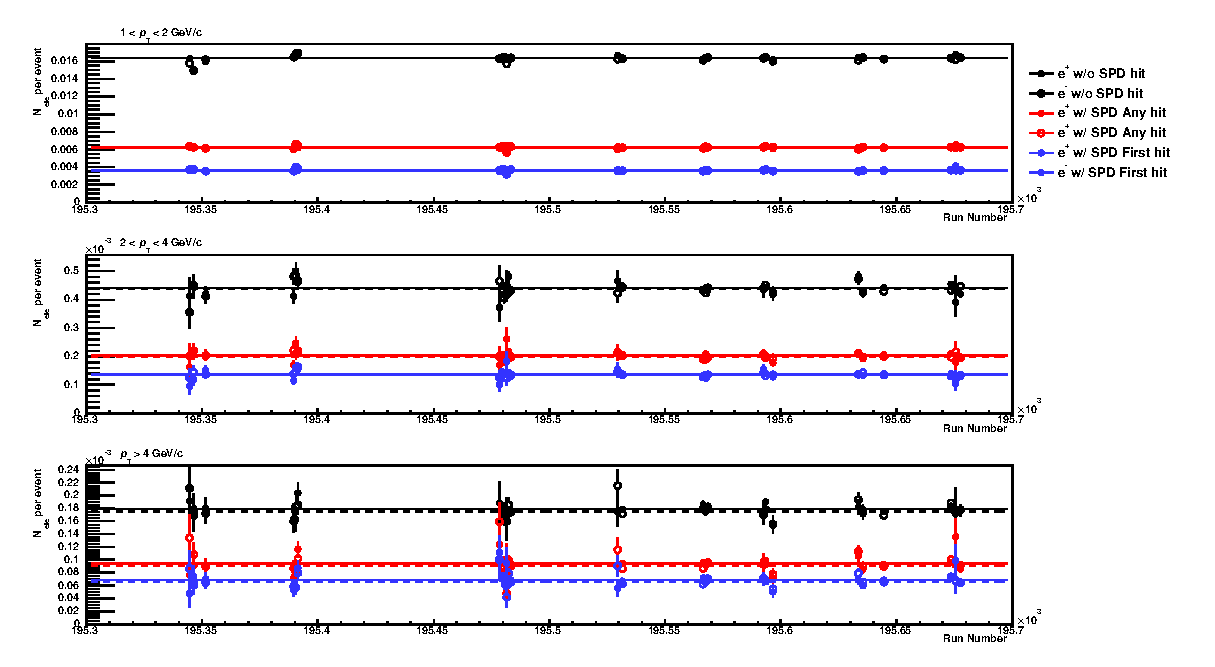
\includegraphics[width=16cm]{chap4/figure/QA/RunbyRunQA_MB.eps}
  \caption{The number of accepted tracks per event after the typical track quality and electron identification cuts for each run.}
  \label{fig_4_runqa_MB}
\end{figure}
\begin{figure}[!h]
  \centering
  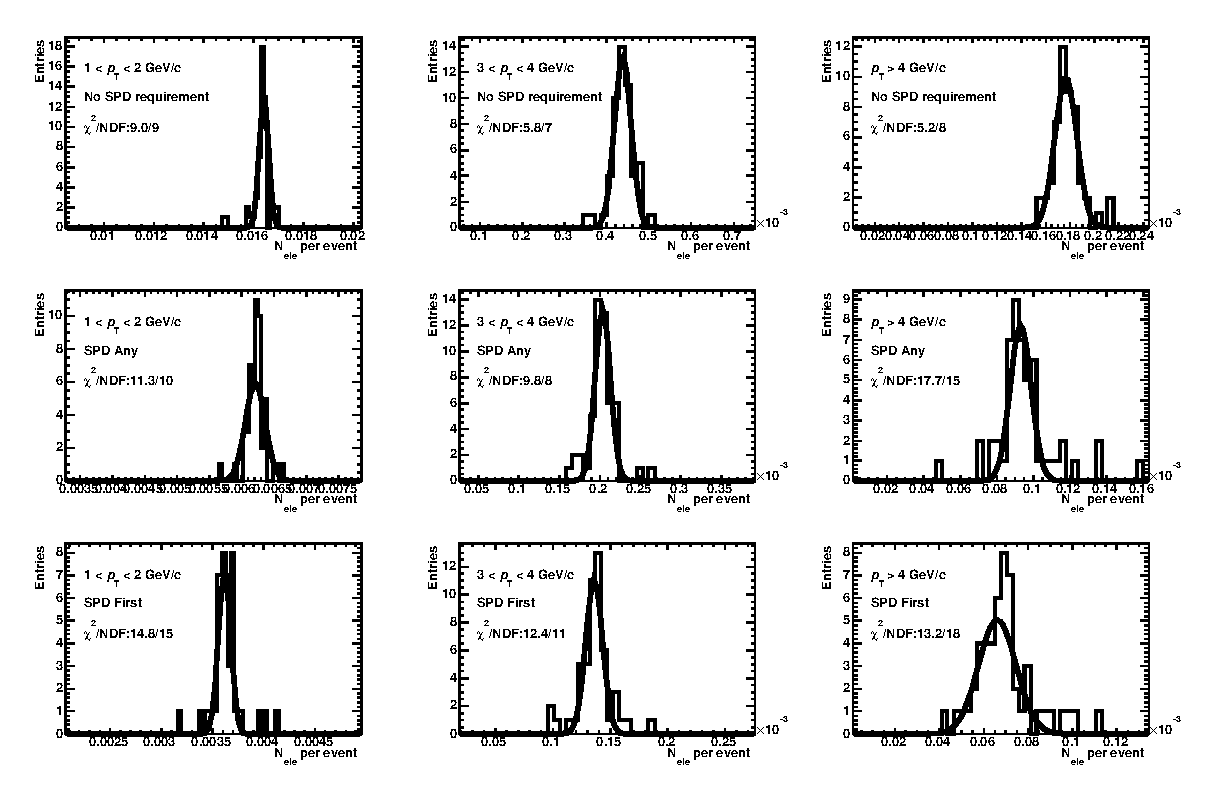
\includegraphics[width=16cm]{chap4/figure/QA/RunbyRunQAPro_MB.eps}
  \caption{The Projection of the number of accepted tracks after the typical track quality and electron identification cuts for each run and the fitting results. The results contain both electron and positron candidates. }
  \label{fig_4_runqapro_MB}
\end{figure}
%The similar check is also done for the TRD triggered data samples. 
%The typical $p_{T}$ range is different from minimum bias samples because the different kinematic ranges are aimed. 
%Some runs show discrepancy in both lower and higher samples. 
%The runs which are out of 3 $\sigmas$ from mean in both $p_{T}$ range are rejected.

%\begin{figure}[!h]
 % \centering
 % 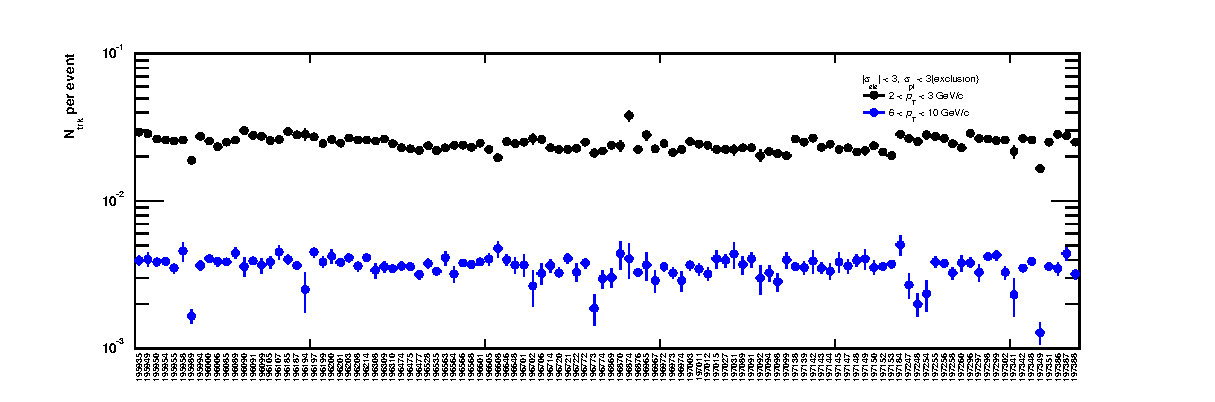
\includegraphics[width=15cm]{chap4/figure/QA/RunByRunPIDQA_TRDTrigger.eps}
 % \caption{The number of accepted track after typical track quality and electron identification cuts for each TRD trigger runs.}
 % \label{fig_4_runqa_Trigger}
%\end{figure}

\section{Track Selection}
\label{sec_4_trackrec}
\subsection{Kinematic Selection}
Figures~\ref{fig_4_legptkin},~\ref{fig_4_legptkin2} show the leg $p_{T}$ distribution of $J/\psi$.
Since $J/\psi$ has the invariant mass of 3.096 GeV/$c^{2}$, both electrons have relatively high $p_{T}$ ($\sim$ 1.5 GeV/c) with large opening angle at low mother $p_{T}$.  
At intermediate mother $p_{T}$, one leg electrons carry a large part of mother's momentum and the other one have smaller momentum up to 0.5 GeV/c. 
In the ALICE central barrel, charged tracks can be reconstructed from $p_{T} > $ 0.2 GeV/c. 
Therefore full momentum space of $J/\psi$ can be covered in this analysis. 
\begin{figure}[!h]
  \centering
  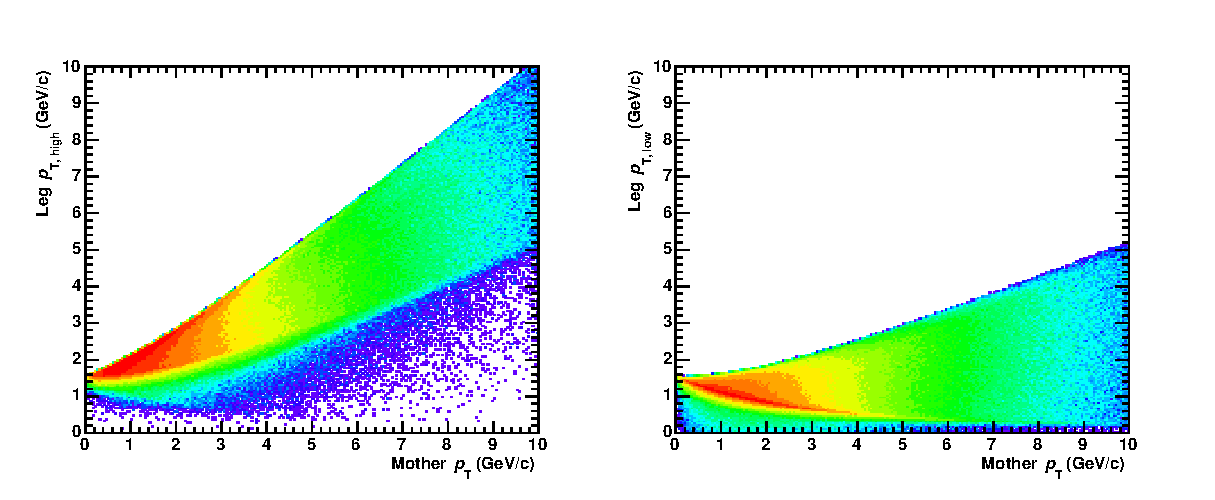
\includegraphics[width=16cm]{chap4/figure/Kinematics/Jpsi_mompt_legpt.eps}
  \caption{ $p_{T}$ distribution of leg electrons with higher $p_{T}$ (Left) and lower $p_{T}$ (Right) from $J/\psi$ decays as a function of mother $p_{T}$ in Monte-Carlo simulation. }
  \label{fig_4_legptkin}
\end{figure}
%\begin{figure}[!h]
%  \centering
%  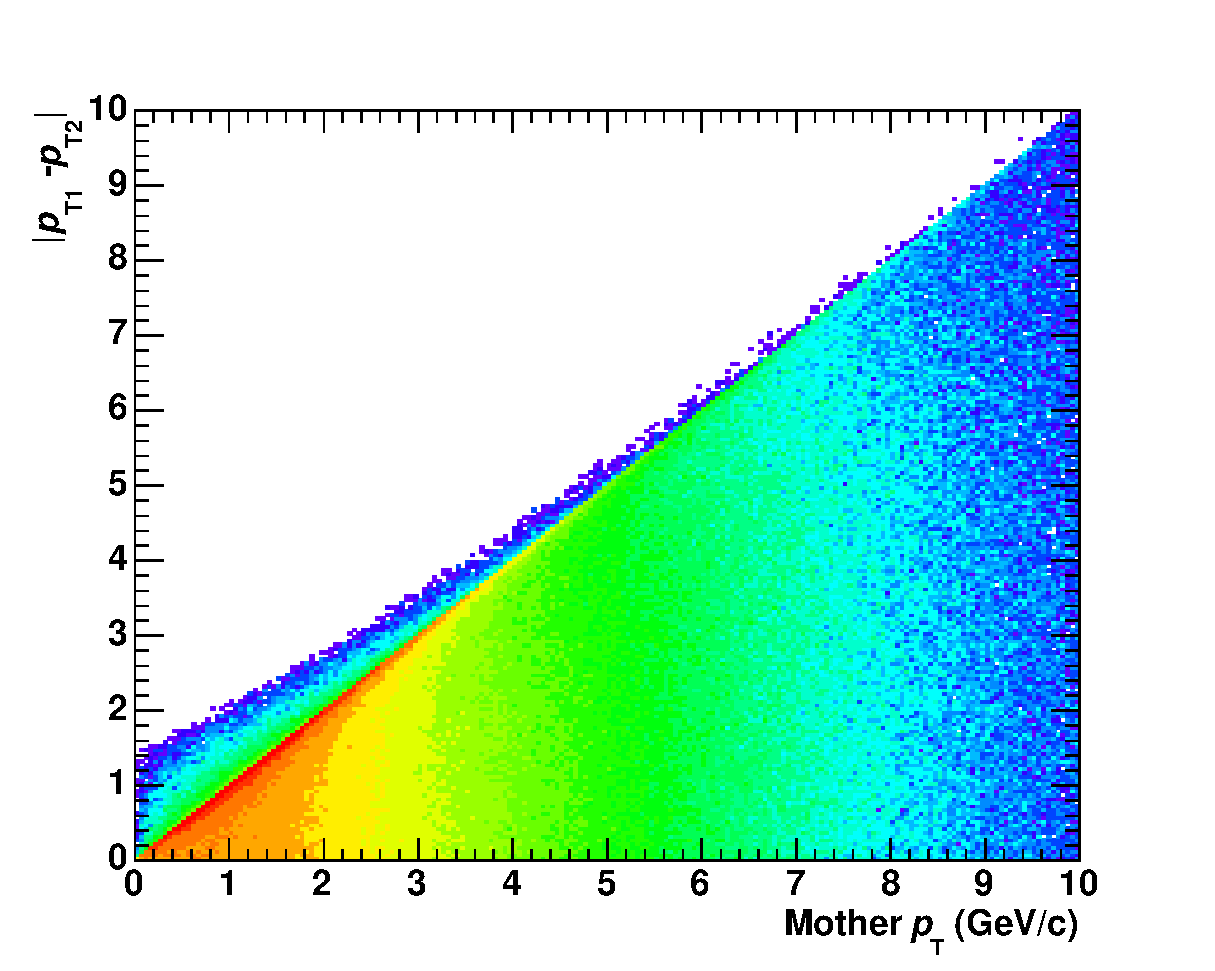
\includegraphics[width=8cm]{chap4/figure/Kinematics/Jpsi_mompt_devlegpt.eps}
%  \caption{Distribution of relative momentum difference between electron-positron pairs from $J/\psi$ decays in Monte-Carlo simulation.}
%  \label{fig_4_legptkin2}
%\end{figure}

In order to keep good signal to background ratio, the combinatorial background generated by electrons from light hadron decays and material conversion is needed to be suppressed sufficiently. 
In this analysis, the following kinematic selection is applied, 
\begin{itemize}
  \item $p^{e}_{T}~>~1~GeV/c$ 
  \item $|\eta^{e}|~<~0.9$
\end{itemize}
In case $p_{T}$ differential analysis, $p^{e}_{T}~>$ 0.8 GeV/c is applied fo 3-5 GeV/c bin to increase the significance. 

Figures~\ref{fig_4_jpsiacce} show the kinematic acceptance of $J/psi$ in Monte-Carlo simulation. 
With the above kinematic selection, full momentum measurement of J/$\psi$ at central region is still valid. 
\begin{figure}[!h]
  \begin{minipage}{0.5\hsize}
    \begin{center}
      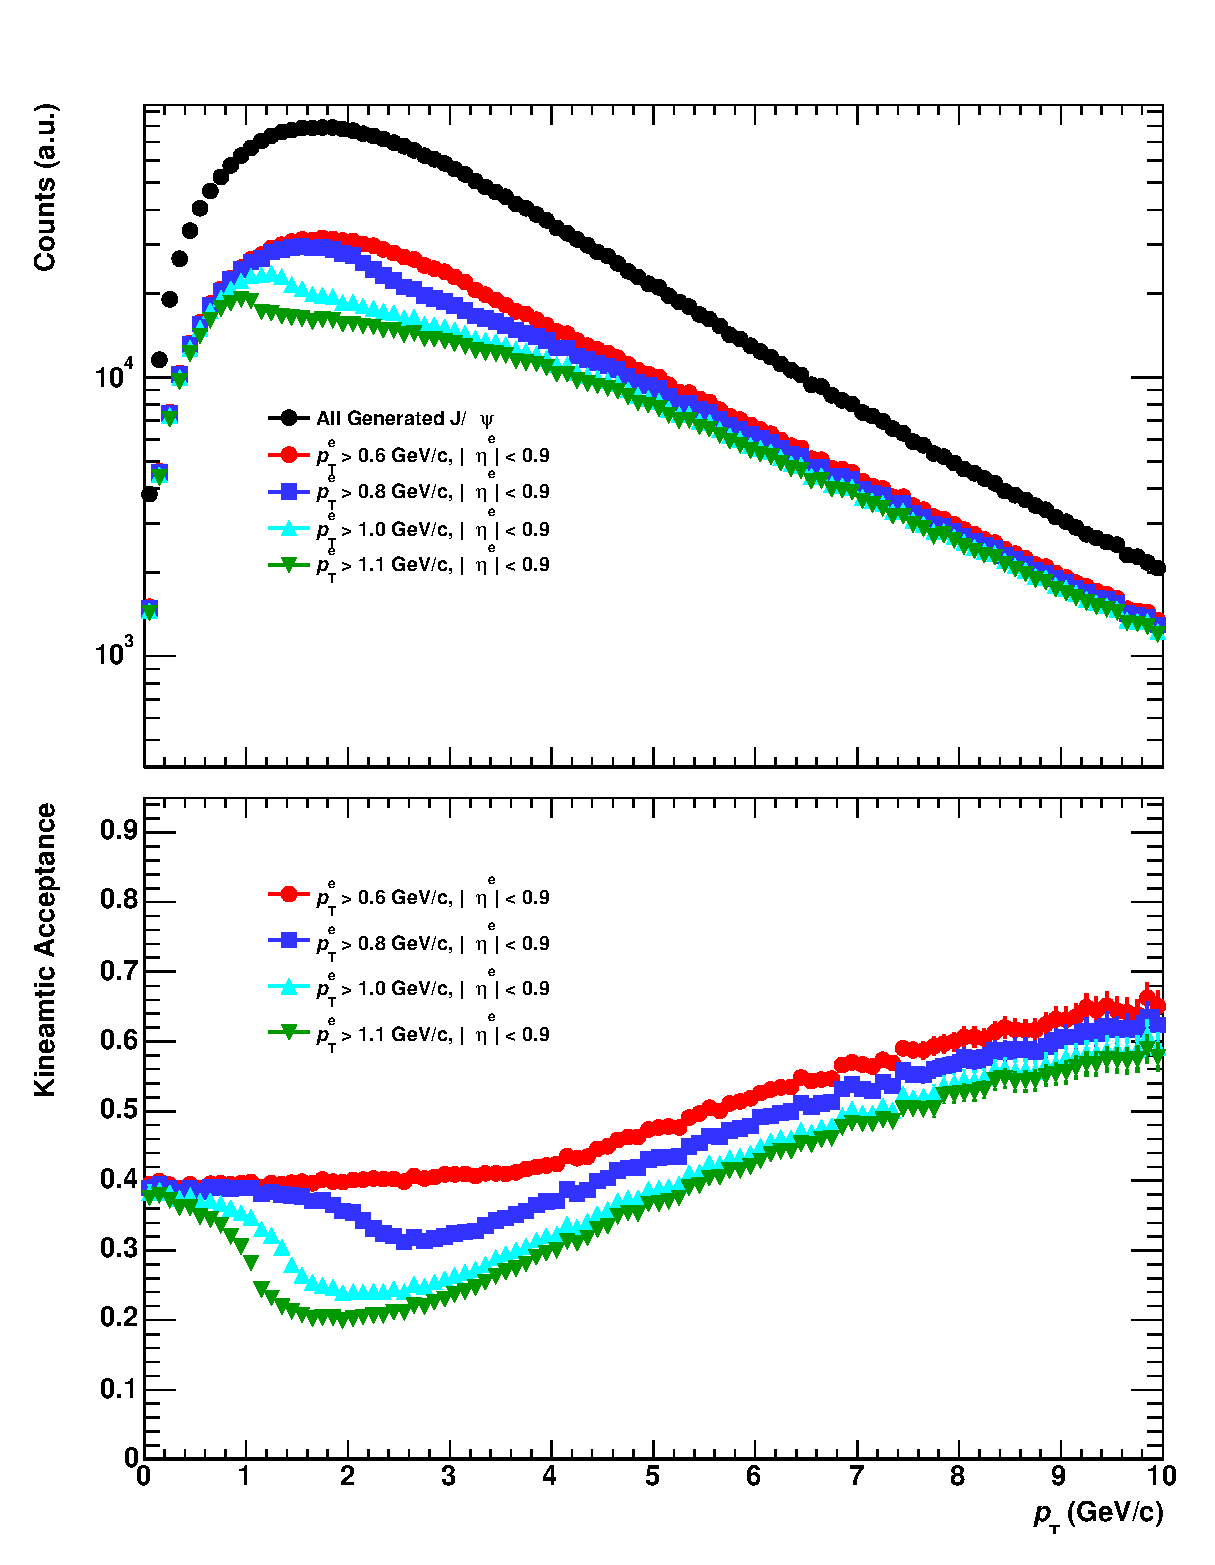
\includegraphics[width=8cm]{chap4/figure//Kinematics/MCJpsi_ptacce.eps}
    \end{center}
  \end{minipage}
  \begin{minipage}{0.5\hsize}
    \begin{center}
      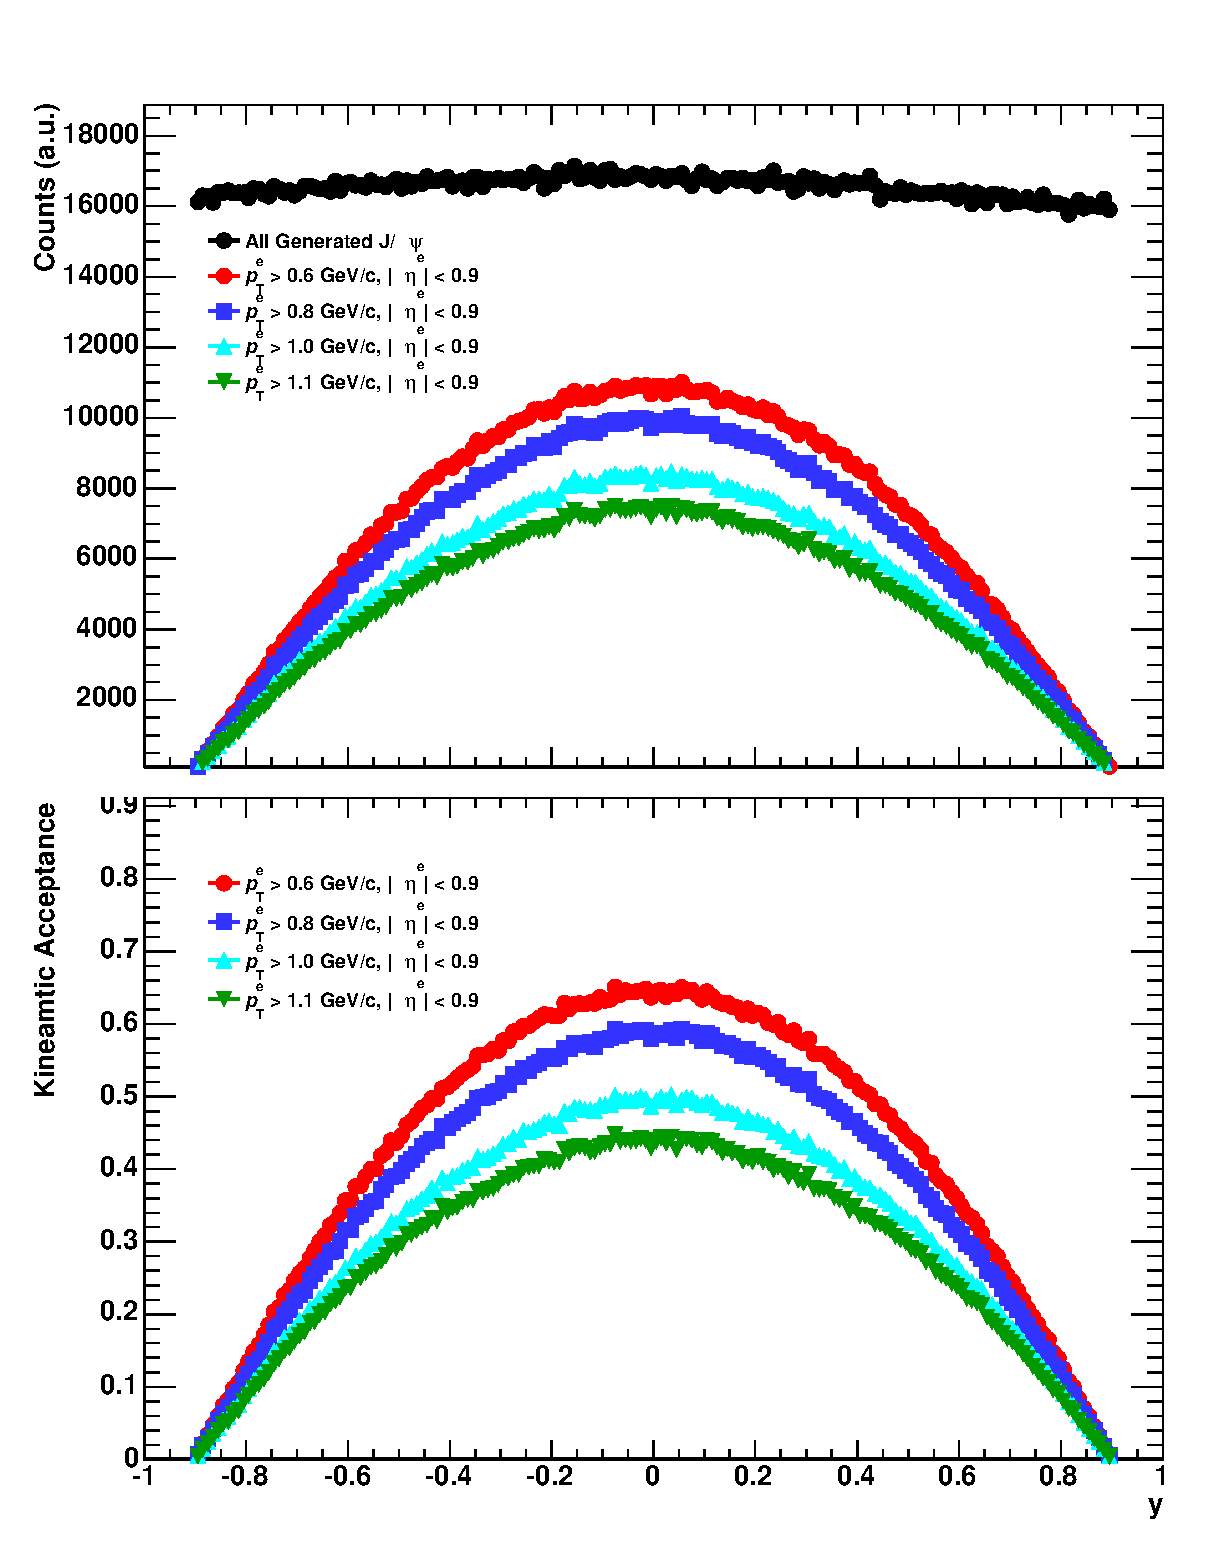
\includegraphics[width=8cm]{chap4/figure//Kinematics/MCJpsi_yacce.eps}
    \end{center}
  \end{minipage}
  \caption{
    Kinematic acceptance for J/$\psi$ as a function of $p_{T}$ (Left) and y (Right) in Monte-Carlo simulation.
  }
  \label{fig_4_jpsiacce}
\end{figure}

\subsection{Track Quality Cuts}
\begin{table}[!htb]
  \centering
  \begin{tabular}{cc} \hline
    Cut   & Value \\ \hline
    Minimum leg $p_{T}$  & $>$ 1 GeV/c \\ \hline
    $|\eta^{e}_{lab}|$  & $<$ 0.9 \\ \hline
    refit  &  ITS and TPC\\ \hline
    The number of TPC clusters (TPC $N_{cls}$) & $>$ 70 \\ \hline
    TPC $\chi^{2}/N_{cls}$ & $<$ 4 \\ \hline
    $|DCA_{XY}|$ & $<$ 1 cm \\ \hline
    $|DCA_{Z}|$ & $<$ 3 cm \\ \hline
  \end{tabular}  
  \caption{Summary of cuts setting for track reconstruction. }
\end{table}
Charged tracks are reconstructed using hits on ITS and TPC in the ALICE detectors as described in Section\ref{sec_3_trackrec}.
In order to select good track samples, ITS and TPC quality cuts are applied. 
All selected tracks are required refit (See Section\ref{sec_3_trackrec}) of ITS and TPC since all electrons from $J/\psi$ are assumed to  come from a primary vertex or produced around primary vertex by feed down from bottom hadrons.
The loose impact parameter cuts for XY plane and Z axis are also applied ($DCA_{XY} <$1 cm, $DCA_{Z} < $3 cm).  
Figure~\ref{fig_4_qa_tpc} show the distribution of the number of TPC clusters and $\chi^{2}$ divided by TPC clusters of electron candidates. 
\begin{figure}[!h]
  \centering
  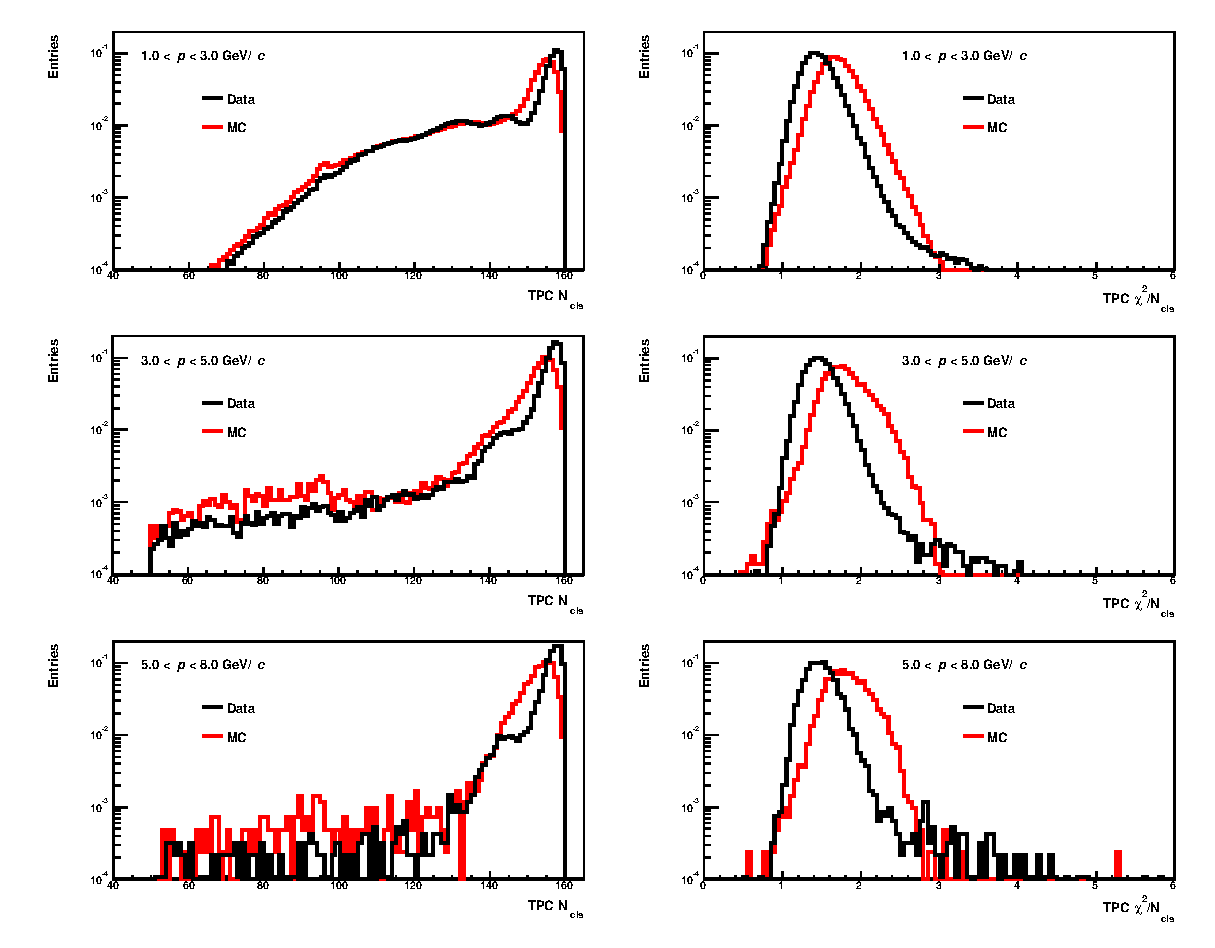
\includegraphics[width=15cm]{chap4/figure/TrackQA/QA_MomBin_tof3_tpc2_tpcpi3_MB.eps}
  \caption{Distribution of the number of TPC clusters (Left) and TPC $\chi^{2}$ divided by the number of TPC clusters (Right) for electron samples in 3 momentum ranges. The balck lines show the result of the real data and the red lines show the result of Monte-Carlo simulation.}
  \label{fig_4_qa_tpc}
\end{figure}
There are clear discrepancies between the experimental data and Monte-Carlo simulation. 
However tracks are required at least 70 clusters out of maximum 159 hits and $\chi^{2}$ per TPC clusters below 4. 
Therefore integrated efficiency is similar between real data and Monte-Carlo. 

\begin{figure}[!h]
  \centering
  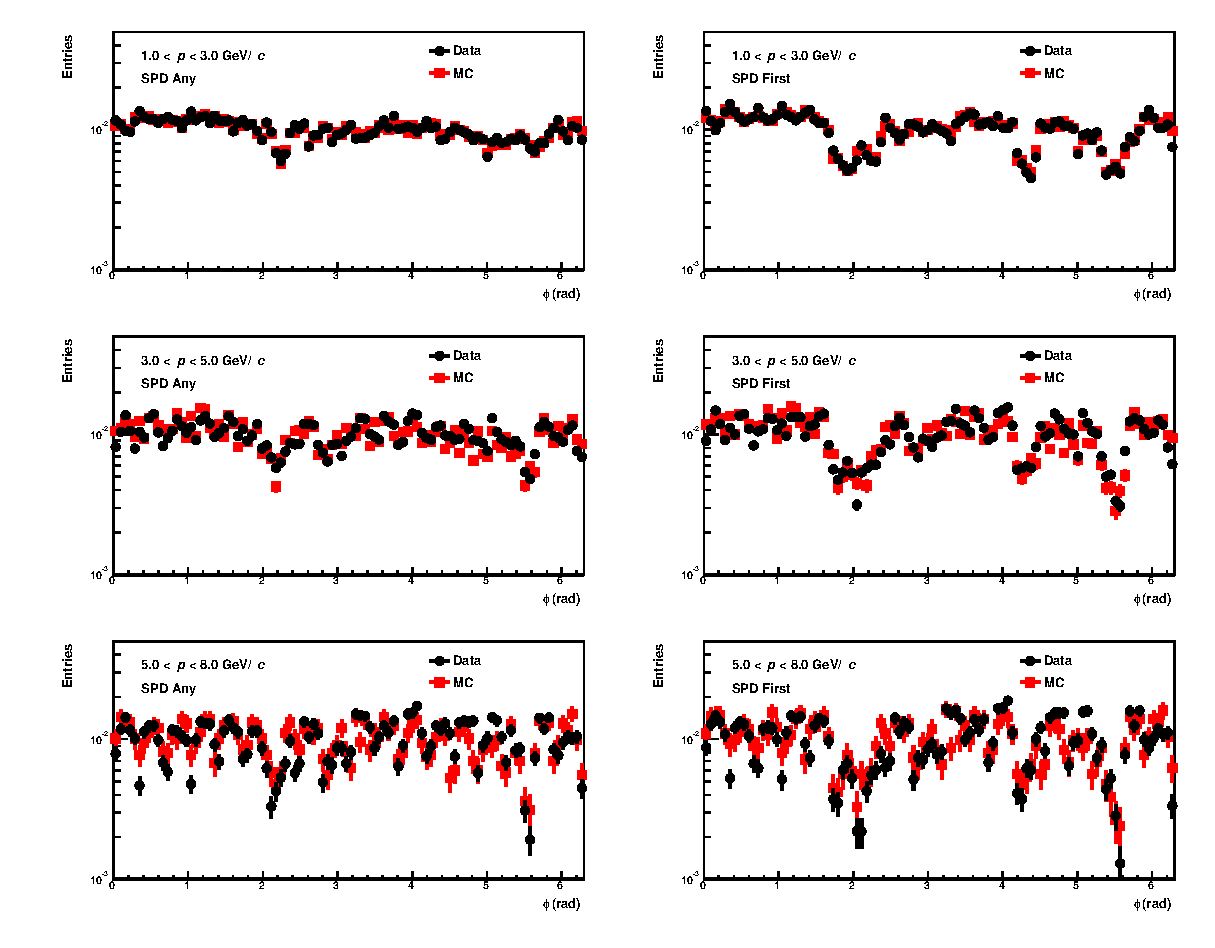
\includegraphics[width=15cm]{chap4/figure/TrackQA/Phi_tof3_tpc2_tpcpi3_MB.eps}
  \caption{$\phi$ distribution of electron samples after SPD Any (Left) and First (Right) requirements. The balck markers show the result of the real data and the red markers show the result of Monte-Carlo simulation.}
  \label{fig_4_qa_phi}
\end{figure}

\begin{figure}[!h]
  \centering
  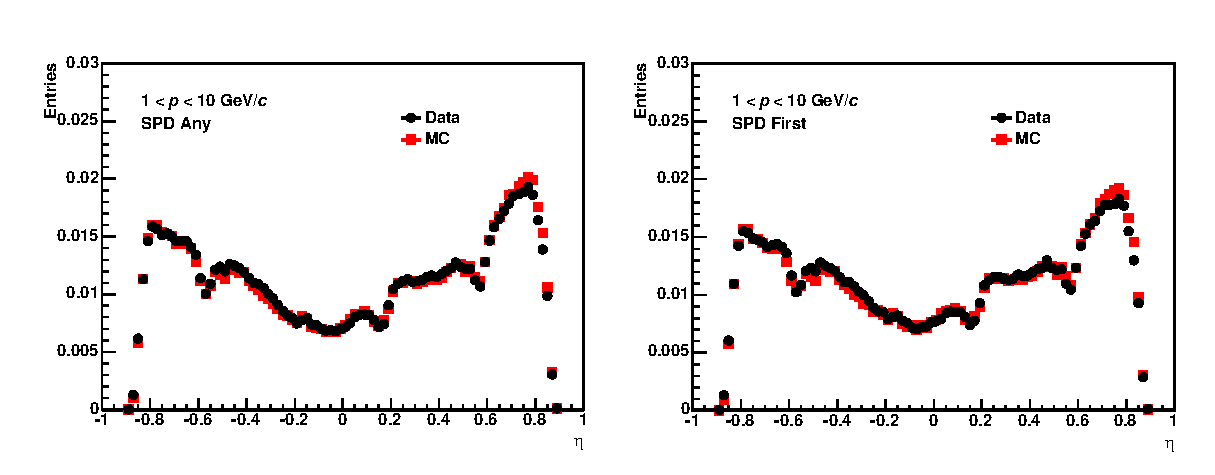
\includegraphics[width=15cm]{chap4/figure/TrackQA/Eta_tof3_tpc2_tpcpi3_MB.eps}
  \caption{$\eta$ distribution of electron samples after SPD Any (Left) and First (Right) requirements. The balck markers show the result of the real data and the red markers show the result of Monte-Carlo simulation.}
  \label{fig_4_qa_eta}
\end{figure}

For the rejection of conversion electrons and out-of-bunch pileup electrons, hits on the SPD layers are required since SPD is the most inner tracking detector and provide a rejection of conversion electrons produced at larger radii. 
SPD also has a fast integration time ($\sim$100 ns) compared to the bunch spacing (200 ns in p-Pb case) and then the contribution from out-of-bunch is negligible by the SPD hit requirement. 
Figures~\ref{fig_4_qa_phi},~\ref{fig_4_qa_eta} show the $\phi$ and $\eta$ distributions of reconstructed tracks after the SPD Any and First requirements. 
SPD Any means at least one hit on SPD layers is required while SPD First means a hit on the first layer of SPD is required. 
There is a good agreement between real data and Monte-Carlo simulations. 
SPD First requirement decrease the electron efficiency but it has an advantage of conversion rejection since almost all conversion electrons which generated outer than SPD first layer can be rejected. 
This SPD hit requirement is tune for each momentum bins considering other cut parameters. 

\section{Electron Identification}
\label{sec_4_eid}
ALICE has many detectors for electron identification in the central barrel.
TOF is useful for the rejection of pion, proton, and kaon below 3 GeV/c. However the matching efficiency between TPC and TOF is not good $\sim$ 70\% due to the dead space and the large patch size of readout. 
TRD also provides a good electron/pion separation above 1 GeV/c but only 12 sectors out of 18 sectors are installed in Run1. 
Therefore, in this analysis, only dE/dx information of TPC is used for electron identification to obtain enough acceptance and detection efficiency. 

For the data driven quality assurance of electron identification, conversion electrons are very useful because we can obtain high purity electron samples with topological pair selections of the secondary decay vertex (V0) using V0-finder. 
V0-finder is used for the reconstruction of secondary decay vertex like $\Lambda$, $K^{0}_{s}$, and conversion electrons. 
Figure~\ref{fig_4_v0finder} shows the schematics of the V0 reconstruction. 
V0-finder calculates the pair DCA for all unlike-sign pairs whose leg tracks has large impact parameters to find the secondary decay pairs during track reconstruction. 
\begin{figure}[!h]
  \centering
  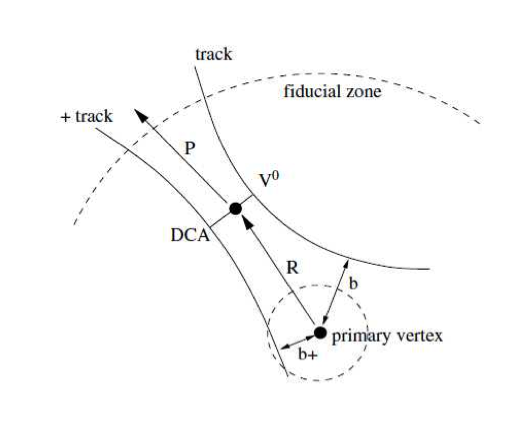
\includegraphics[width=6cm]{chap4/figure/PID/v0-finder.eps}
  \caption{Schematics of V0-finder. }
  \label{fig_4_v0finder}
\end{figure}

Since Conversion electrons are produced from real photons in the detectors or beam pipes, their pair invariant mass is zero (very small opening angle) and they pass through the detectors in the constant magnetic field.  
The left panel of Fig.~\ref{fig_4_almenterosandpurity} shows the Almenteros-Podolanski plot in p-Pb collisions.
The x-axis of it is longitudinal momentum asymmetry. 
The y-axis $q_{T}$ is defined as projection of the momentum of daughters with respective to the mother $p_{T}$ direction ($\it{p}\times sin\theta_{mother-daughter}$). 
Conversion electrons localize around zero due to the mass less photon decays.  
%They also have unique other topological features such as their pair plane angle to the magnetic field. 
The cut setting for conversion electron identification is summarized in Table.~\ref{table_convcut}.
\begin{table}[!h]
  \centering
  \begin{tabular}{cc} \hline
    Cut  & Value \\ \hline
    V0 status  & On-The-Fly \\ 
    Minimum leg $p_{T}$  & $>$ 0.05 GeV/c \\ 
    TPC $N_{cls}$/$N_{findable}$ & $>$ 0.6 \\ 
    $R_{conv}$  & 5 $<$ R $<$ 180 cm \\
    $Z_{conv}$  & Z $<$ 240 cm \\ 
    $DCA_{pair}$  & $<$ 0.25 cm\\ 
    $\Psi_{pair}$  & $<$ 0.05 \\ 
    $(\alpha/0.95)^{2}~+~(q_{T}/0.05)^{2}$  & $<$ 1 \\ 
    $m_{ee}$  & $<$ 50 MeV/$c^{2}$ \\ \hline
  \end{tabular}  
  \label{table_convcut}
  \caption{Summary of the conversion electron selections. }
\end{table}

Conversion electrons can be selected with high purity $>$ 98\% in all $p_T$ region as shown in the right panel of Fig.~\ref{fig_4_almenterosandpurity}. 
The purity is extracted by the full Monte-Carlo simulation.  
\begin{figure}[htbp]
 \begin{minipage}{0.5\hsize}
  \begin{center}
  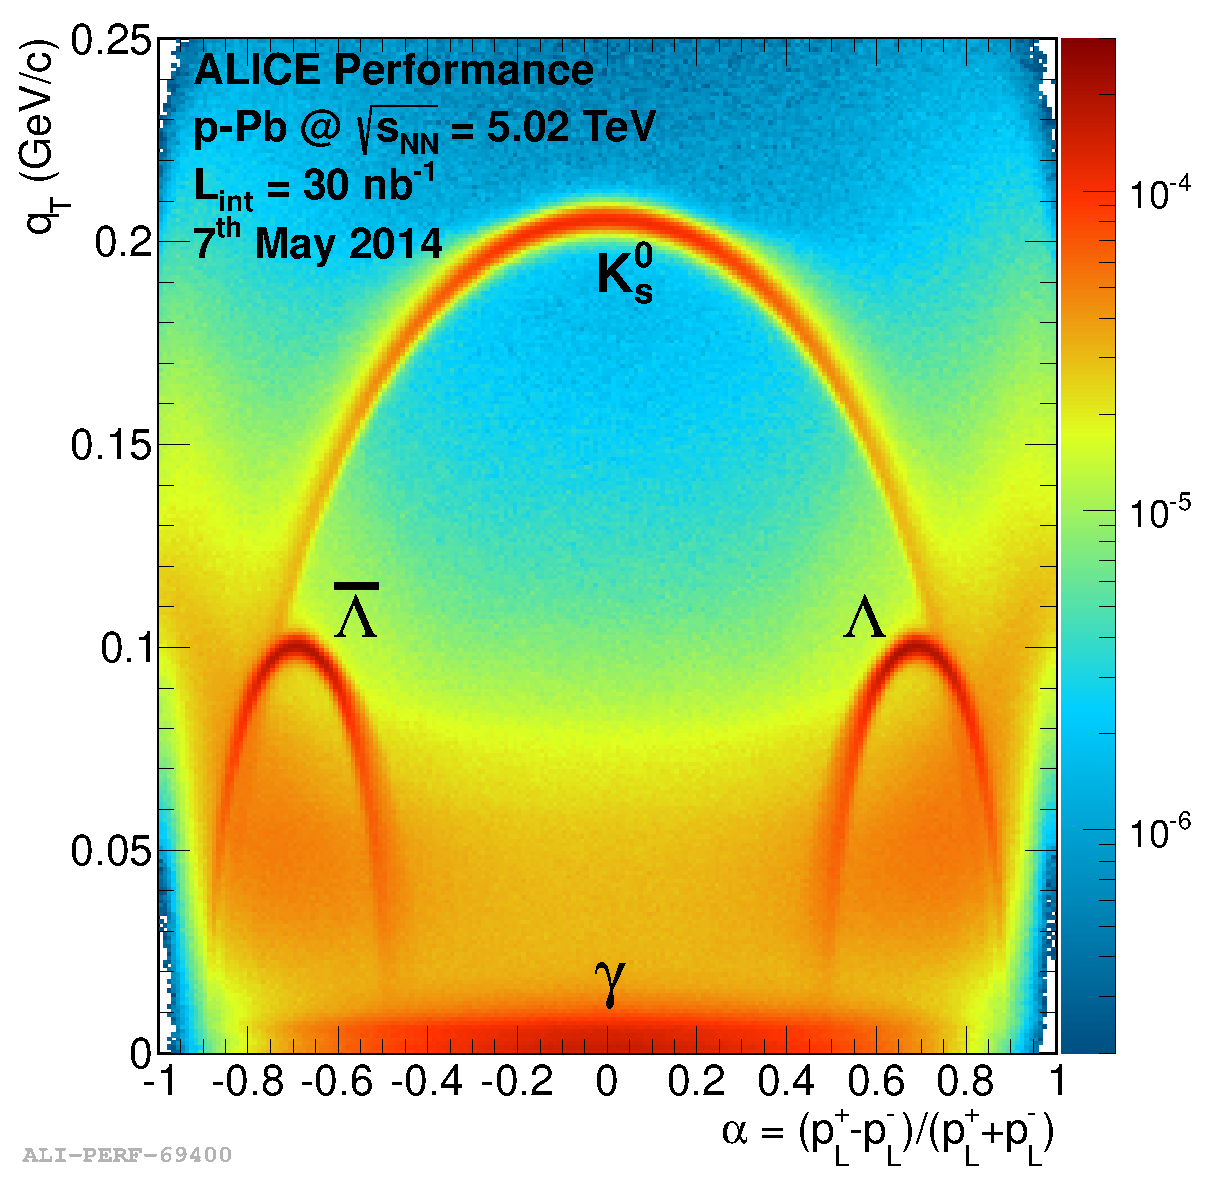
\includegraphics[width=6cm]{chap4/figure/Conversion/ArmenterosPlot_pPb.eps}}
  \end{center}
 \end{minipage}
 \begin{minipage}{0.5\hsize}
  \begin{center}
  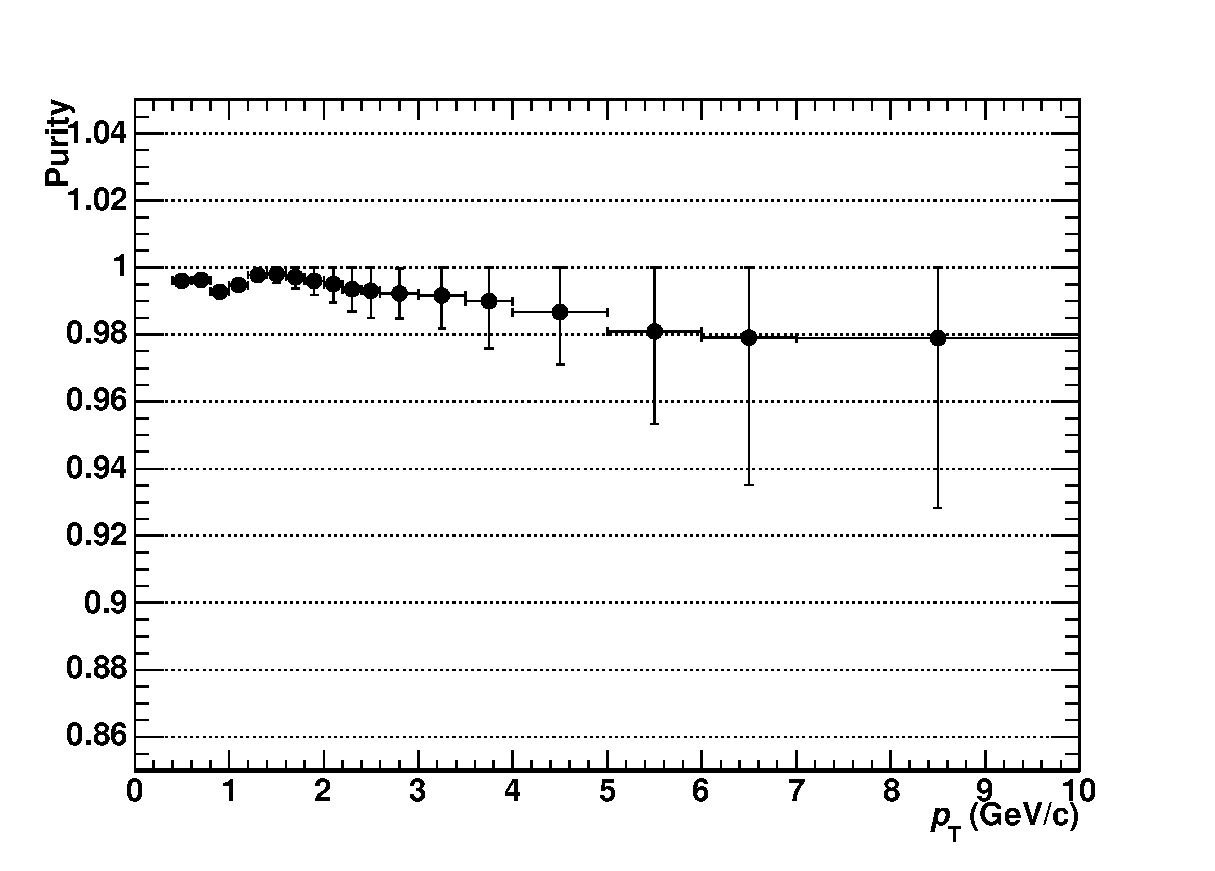
\includegraphics[width=8cm]{chap4/figure/Conversion/SingleV0Cut_ElePurity_Pt.eps}
  \end{center}
 \end{minipage}
  \caption{Almenteros-Podolanski plot in p-Pb collision at $\sqrt{s_{NN}}=$5.02 TeV (Left) and the electron purity of conversion samples extracted by the full Monte-Carlo simulation.  }
  \label{fig_4_almenterosandpurity}
\end{figure}

TPC dE/dx follows the Bethe-Bloch formula as described in Section~\ref{sec_3_pid}. 
The ALEPH TPC introduced the useful parametrization to match the Bethe-Broch curve from the real data. 
The expected dE/dx value is approximated by the following equation, 
\begin{equation}
  \langle \frac{dE}{dx} \rangle_{expected} = f(\beta \gamma) = \frac{P_{1}}{\beta^{P_{4}}}\big( P2-\beta^{P_{4}}-ln(P_{3}+\frac{1}{(\beta\gamma)^{P5}}) \bigr)
\end{equation}
where, P, P2, P3, P4, and P5 are the parameters called as ALEPH parameters. These ALEPH parameters and the width of the electron band ($\sigma_{ele}$) are tuned to the real data and the black curves in Fig.~\ref{fig_3_tpcpid} show the mean point of each particle species after the tuning in p-Pb collisions. 
%The banumber of $sigma_{ele}$ is calculated with the following equation, 
%\begin{equation}
%  \rm{TPC~ n}\sigma_{ele} = \frac{\frac{dE}{dx}_{measured}-\langle \frac{dE}{dx}_{ele}\rangle _{expected}}{\sigma}
%\end{equation}


\begin{figure}[htbp]
 \begin{minipage}{0.5\hsize}
  \begin{center}
  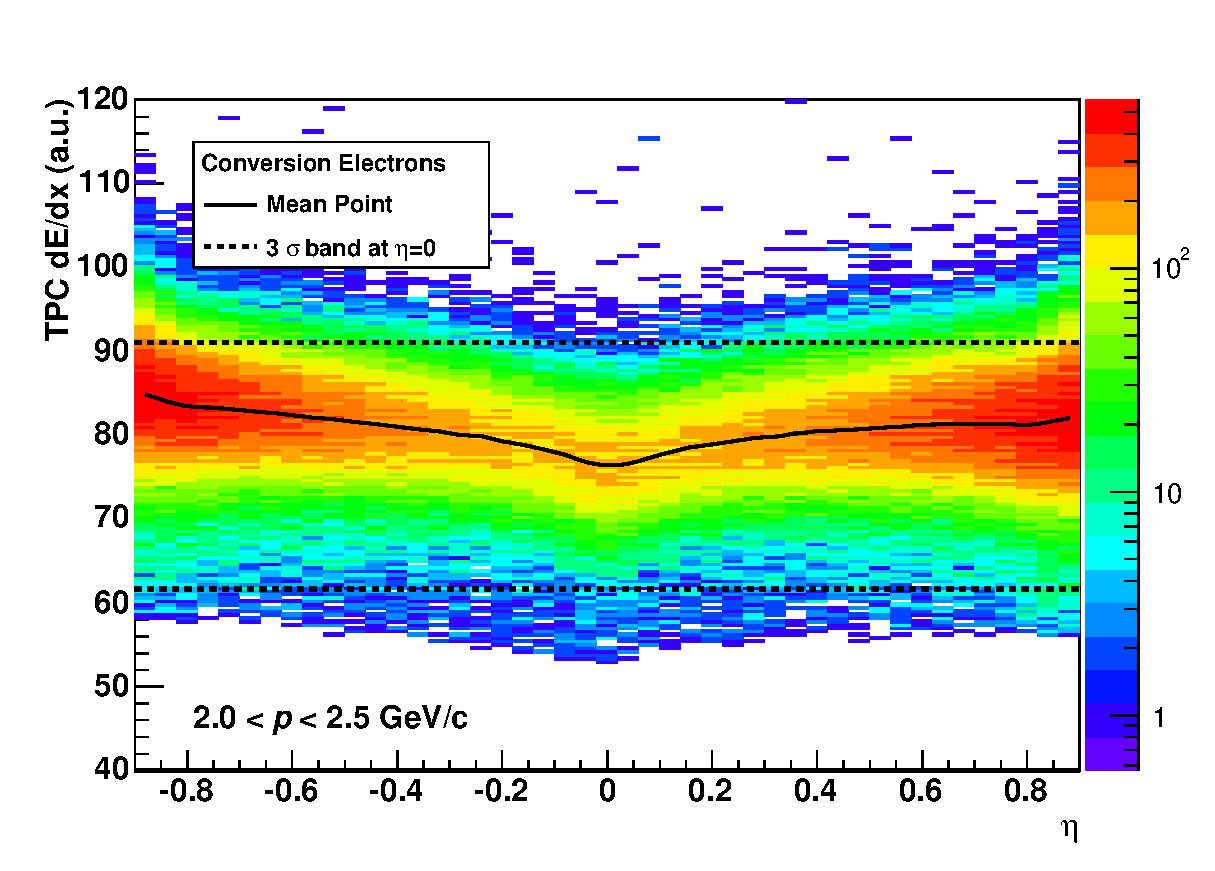
\includegraphics[width=8cm]{chap4/figure/PID/RawTPCdEdxforConv_MB.eps}
  \end{center}
 \end{minipage}
 \begin{minipage}{0.5\hsize}
  \begin{center}
  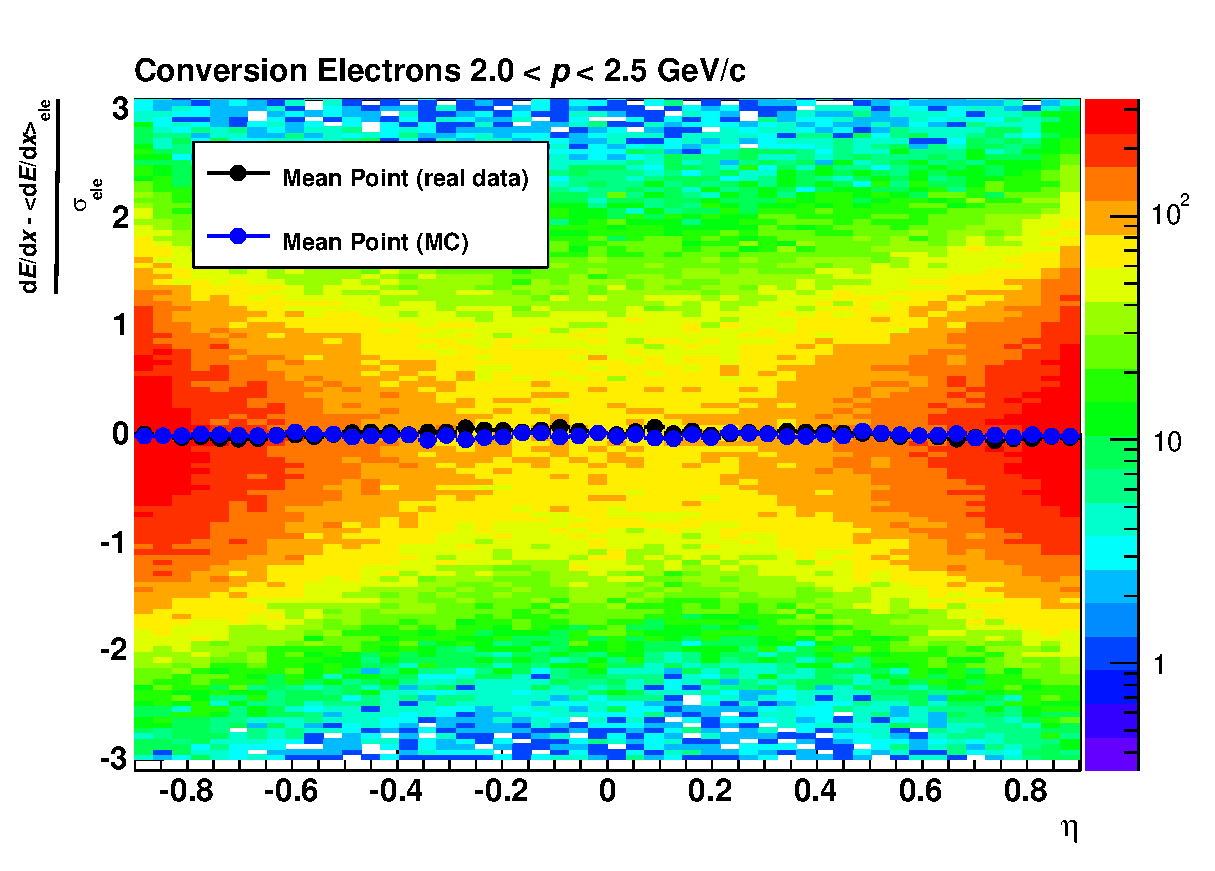
\includegraphics[width=8cm]{chap4/figure/PID/TPCNSigmaforConv_MB.eps}
  \end{center}
 \end{minipage}
  \caption{$\eta$ dependence of the raw TPC dE/dx and the TPC n$\sigma_{ele}$ distribution after 3-D correction for conversion electrons in p-Pb collisions (Left).}
  \label{fig_4_tpcdedxforconv}
\end{figure}

The left panel of Fig.~\ref{fig_4_tpcdedxforconv} shows the $\eta$ dependence of raw TPC dE/dx signal for conversion electrons. 
Due to the difference of path length, deposited charge distribution has strong $\eta$ dependence. 
In order to treat with eID values uniformly in the acceptance, 3D-spline ($p_{T}$, $\eta$, $\phi$) function is generated and the corrected TPC PID value is obtained by poisson smearing. 
The right panel of Fig.~\ref{fig_4_tpcdedxforconv} shows the $\eta$ dependence of TPC n$\sigma_{ele}$ distribution after 3-D correction.  
The distribution shows the flat shape as a function of $\eta$.  
Figure~\ref{fig_4_tpc_pidfit} shows the quality of the signal shape fitting. 
The good agreement between real data and Monte-Carlo simulation as a function of $\it{p}$ is obtained. 
\begin{figure}[!h]
  \centering
  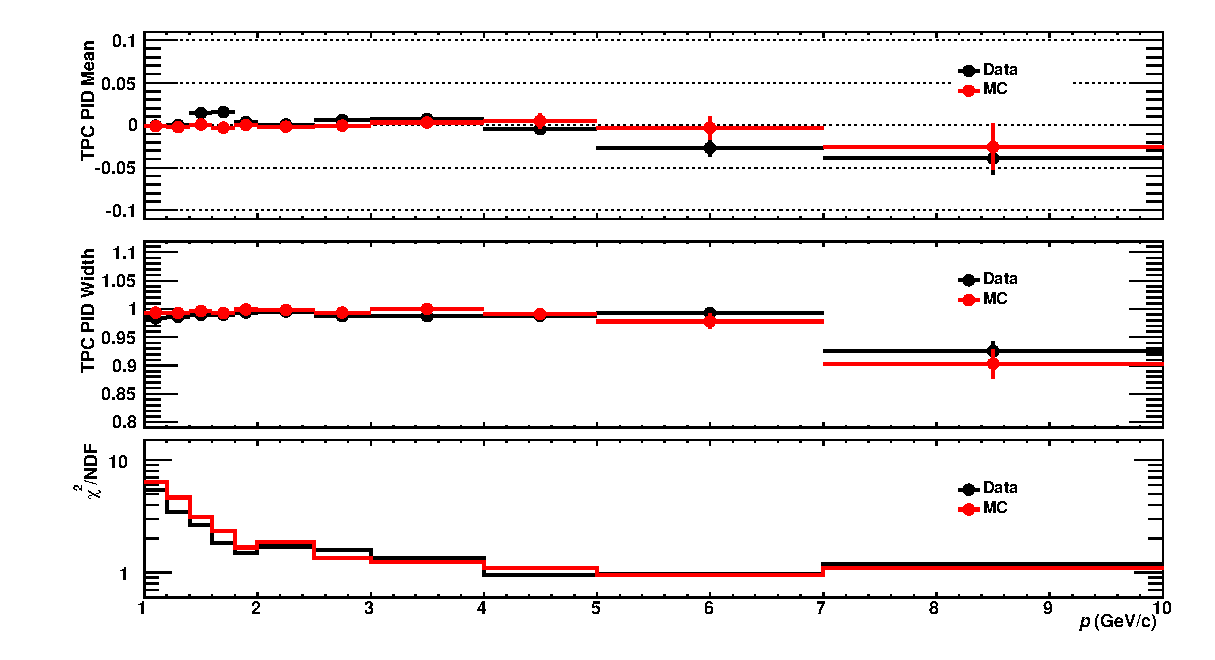
\includegraphics[width=15cm]{chap4/figure/PID/ConvFit_AddEtaCorr_MB.eps}
  \caption{Quality of the gaussian fitting to TPC n$\sigma$ distribution of conversion electrons in p-Pb. The black markers show the results of real data and the red markers show the results of Monte-Carlo simulation.}
  \label{fig_4_tpc_pidfit}
\end{figure}

As a first step of electron identification, all tracks with dE/dx within 3 $\sigma_{ele}$ are selected. 
The left panel of Fig.~\ref{fig_4_tpcnsigmacut} shows the TPC n$\sigma_{ele}$ distribution as a function of $\it{p}$ after the electron inclusion cut. 

%Large proton and pion contribution still exist. 
Large hadron contamination still exist with only inclusion cut mainly from pion and proton. 
\begin{figure}[htbp]
 \begin{minipage}{0.5\hsize}
  \begin{center}
  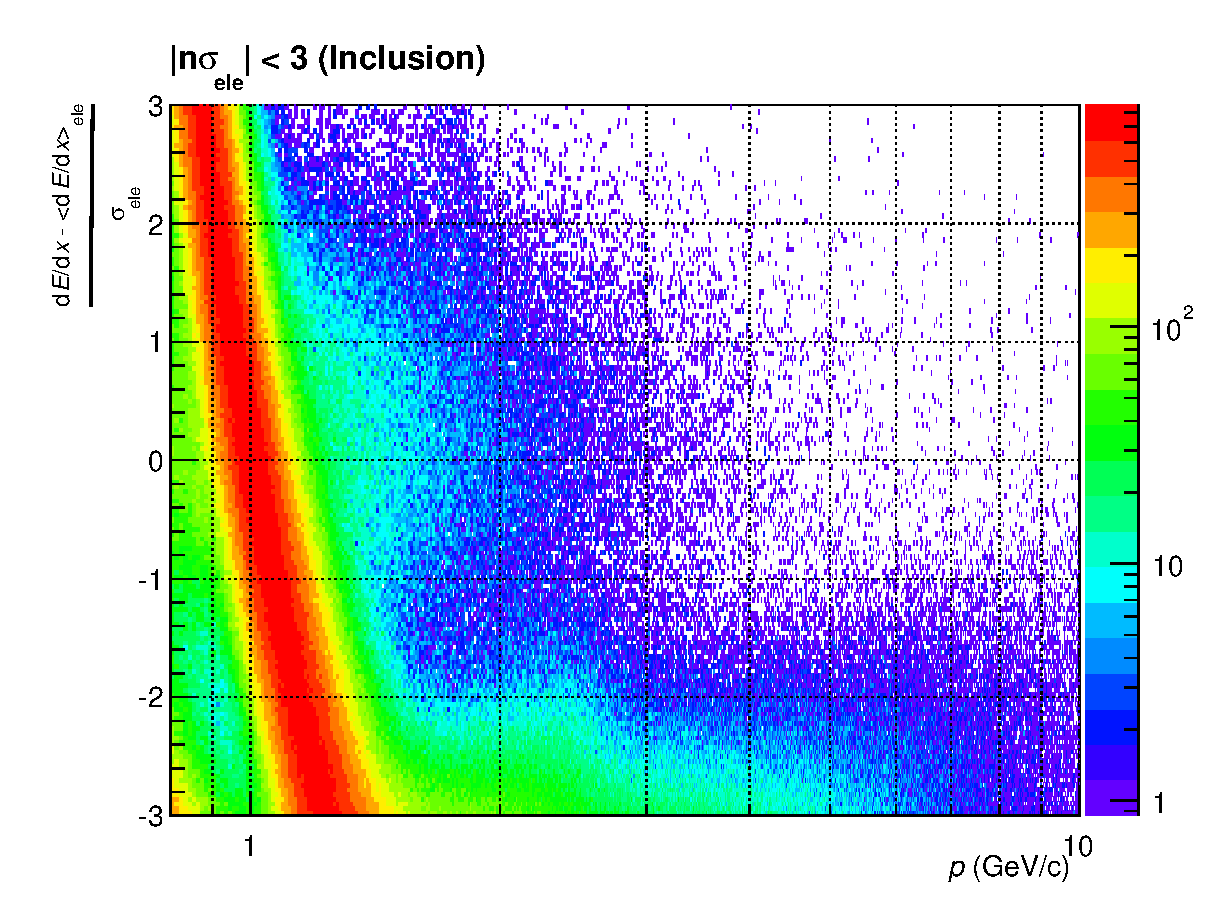
\includegraphics[width=8cm]{chap4/figure/PID/TPCNSigma_AfterInclusion_MB.eps}
  \end{center}
 \end{minipage}
 \begin{minipage}{0.5\hsize}
  \begin{center}
  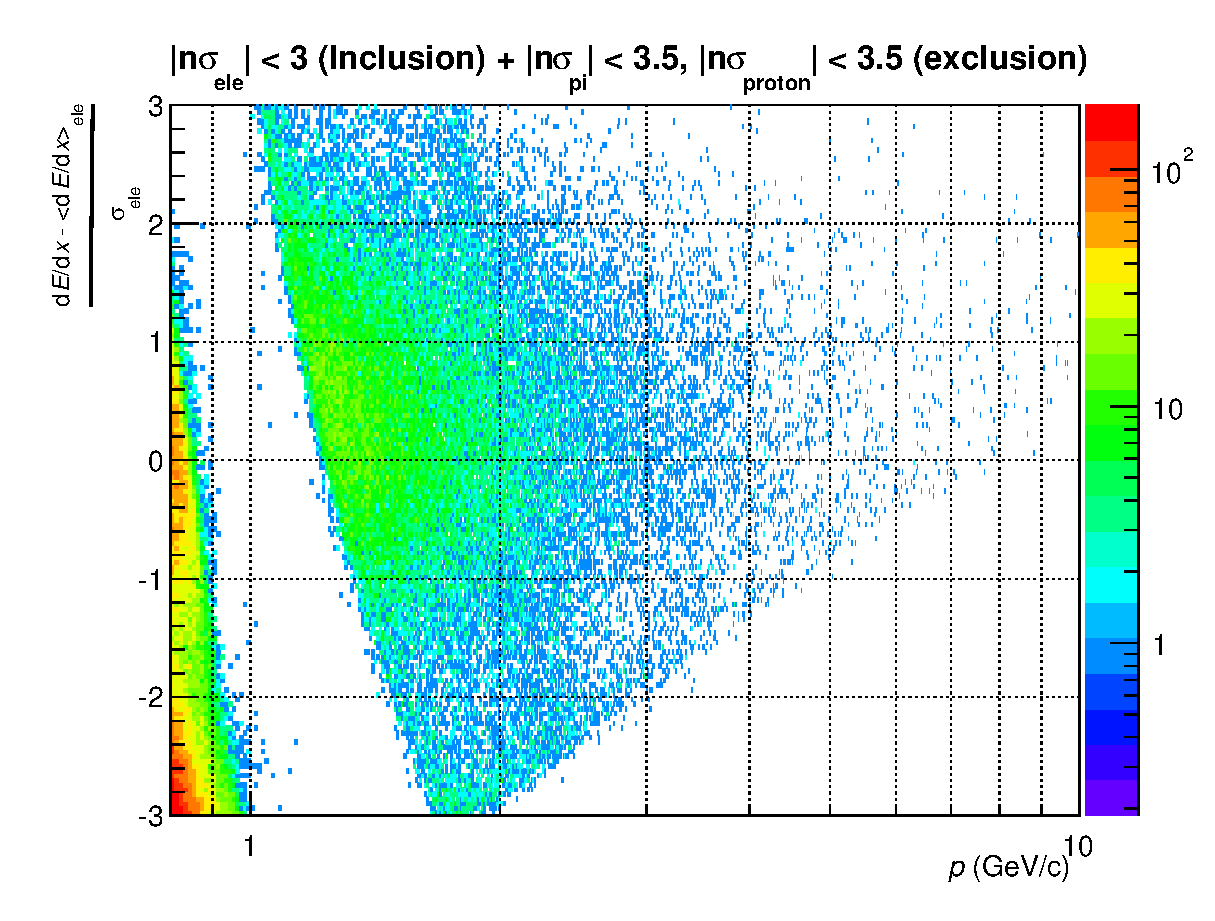
\includegraphics[width=8cm]{chap4/figure/PID/TPCNSigma_AfterExclusion_MB.eps}
  \end{center}
 \end{minipage}
  \caption{TPC n$\sigma_{ele}$ distribution as function of $p$ without hadron exclusion cuts (Left) and with hadron exclusion cuts (Right) in p-Pb collisions.}
  \label{fig_4_tpcnsigmacut}
\end{figure}
The proton band of TPC dE/dx across the electron band around 1 GeV/c.  
Pion and electron bands become merged at higher $p_{T}$ and hadron contamination extremely increases.   

%\begin{figure}[!h]
%  \centering
%  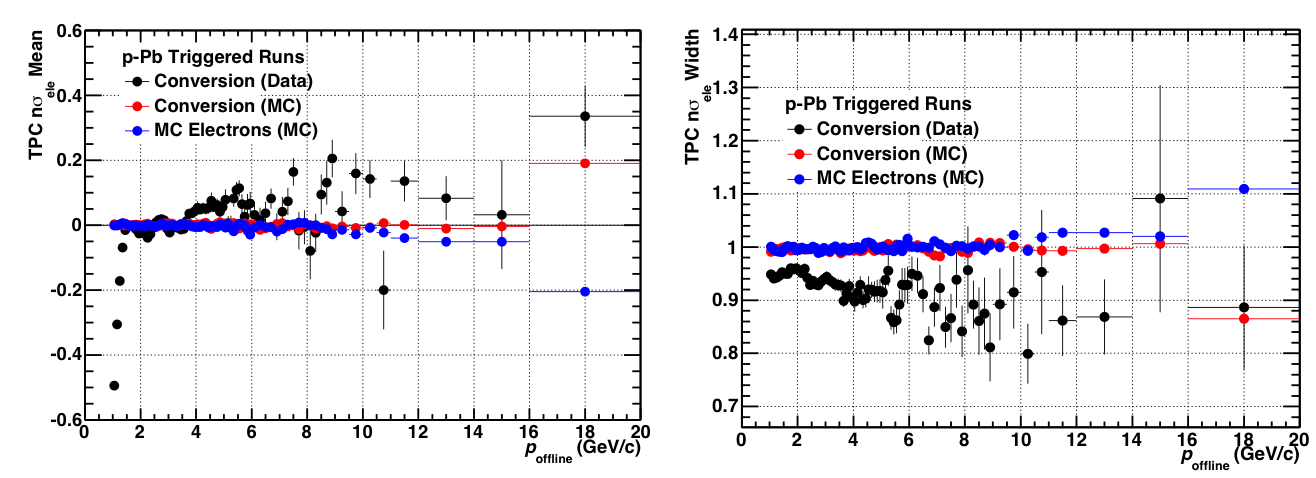
\includegraphics[width=15cm]{chap4/figure/PID/TPCMeanWidth_Ele.png}
%  \caption{Momentum dependence of TPC dE/dx in p-Pb collision at $\sqrt{s_{NN}}=$5.02 TeV.}
%  \caption{Mean and width of gaussian fitting for TPC dE/dx of electrons in p-Pb collision at $\sqrt{s_{NN}}=$5.02 TeV.}
%  \label{fig_4_tpc_mean}
%\end{figure}
%
%\begin{figure}[!h]
%  \centering
%  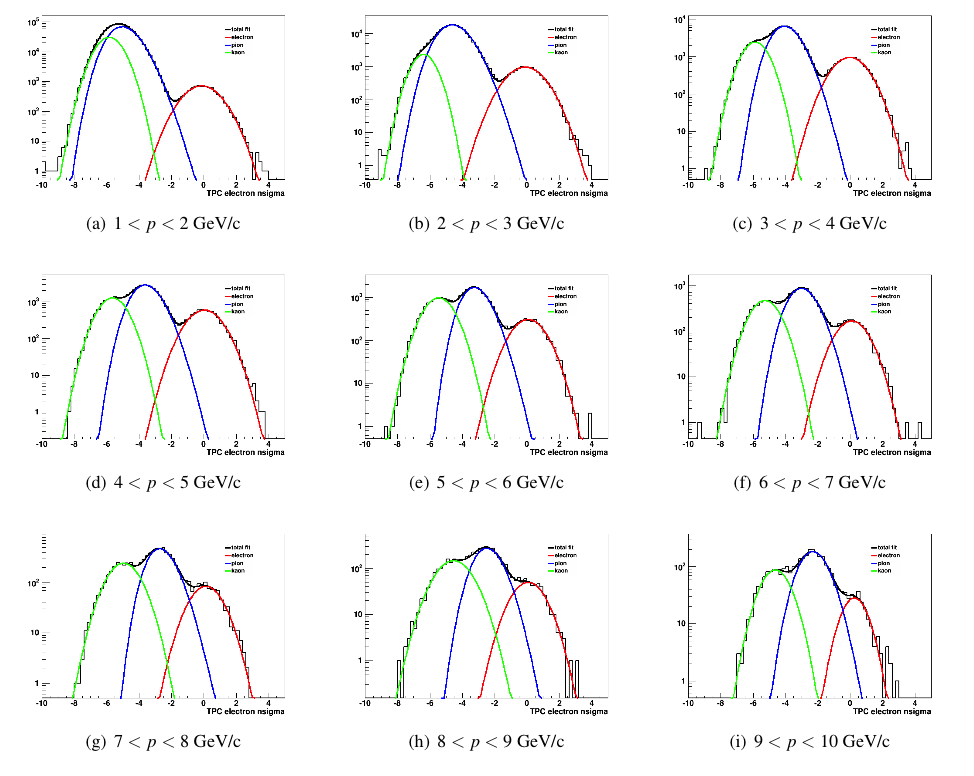
\includegraphics[width=15cm]{chap4/figure/PID/TPCdEdx_MB.png}
%  \caption{Momentum dependence of TPC dE/dx in p-Pb collision at $\sqrt{s_{NN}}=$5.02 TeV.}
%  \label{fig_4_tpc_dedx_momdep}
%\end{figure}

\begin{figure}[htbp]
% \begin{minipage}{0.5\hsize}
  \begin{center}
  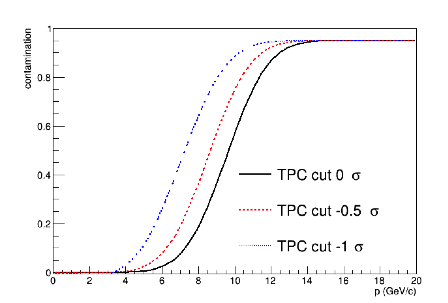
\includegraphics[width=10cm]{chap4/figure/PID/hadroncontami_MB.png}
  \label{fig_4_contami}
  \caption{Electron inclusion cut dependence of pion contamination as a function of $p$ in p-Pb collisions.}
  \end{center}
\end{figure}
Figure~\ref{fig_4_contami} shows n$\sigma_{ele}$ cut dependence of the pion contamination as a function of $p$. 
The electron and pion contributions are estimated by the fitting of gaussian and landau$times$gaussian functions from real data. 
The pion contamination increases rapidly above the momentum threshold depending on the inclusion cut value.
It is described by the erf function and causes the large combinatorial background pairs in $e^{+}e^{-}$ pairs. 
To suppress the rapid rising of hadron contamination, not only the electron inclusion cut but also pion and proton exclusion cuts are applied. 
The right panel of Fig.\ref{fig_4_tpcnsigmacut} shows the examples of TPC dE/dx distribution when pion and proton exclusion cuts within 3 $\sigma$ are applied.  
There are still non-negligible contribution of pion and proton but their contribution is keep below 10\% in all momentum range and it is acceptable for the signal extraction of $J/\psi$ signals. 

 %\end{minipage}
 %\begin{minipage}{0.5\hsize}
 % \begin{center}
\begin{figure}[htbp]
  \begin{center}
    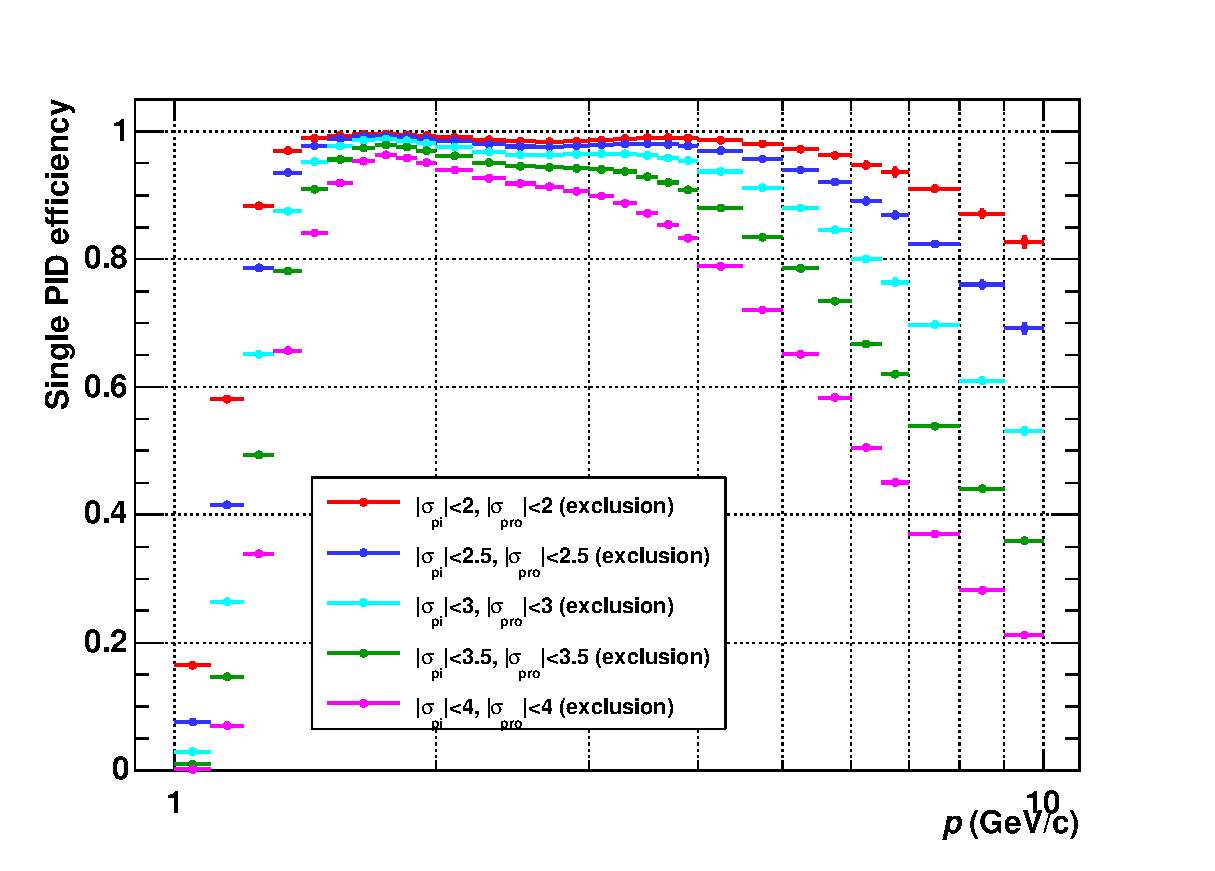
\includegraphics[width=12cm]{chap4/figure/PID/SinglePIDEff_LHC13d10.eps}
  \end{center}
  % \end{minipage}   
  \label{fig_4_pideff}
  \caption{Hadron exclusion cut dependence of single electron identification efficiency in p-Pb collisions.}
\end{figure}

The hadron exclusion cut decrease electron efficiency in particular the lower limit and higher $p_{T}$. 
Figure~\ref{fig_4_pideff} shows single electron PID cut as a function of $p$. 
The final cut setting is tuned in the each momentum bins of $J/\psi$ to increase the significance taking into account the SPD hit requirement.



\section{Rejection of Conversion Electrons}
\label{sec_4_convref}
Conversion electrons are main source of electron candidates in all $p_{T}$ region.
Hit on the most inner detector (SPD) significantly decrease conversion rejection generated at larger radii than SPD.
However, they still account for 25\% of selected electrons at $\it{p}_{T} =$ 2 GeV/c estimated by Monte-Carlo simulation.  

V0-finder described in Section\ref{sec_4_eid} is powerful tool for conversion tagging. 
Monte-Carlo simulation confirms V0-finder reject conversion electrons by a factor of 67\% without any lack of signal electrons. 
At the $J/\psi$ mass, signal to background ratio is improved by a factor 50\%. 

\section{Signal Extraction}
\label{sec_4_signalextraction}
In this analysis no pair cut is applied and the invariant mass is calculated for all electron-positron pairs. 
The background subtraction is crucial part for the precision of raw yield extraction.  

\subsection{Background Subtraction}
The unlike-sign pairs around $J/\psi$ pairs contain the following contribution, 
\begin{description}
  \item{-} $J/\psi$ signal
  \item{-} Correlated $c\bar{c}$ and $b\bar{b}$ decay pairs
  \item{-} Combinatrial pairs from different mother hadrons or conversion photons
  \item{-} Correlated pairs from same or back-to-back jet cone
\end{description}
The main source of the background is combinatorial pairs. 
The combinatorial background can be estimate via event mixing technique. 
Like-sign pairs in same events include not only combinatorial background but also correlated background like jet pairs, and bottom pair decays. 
Therefore more reasonable shape of the background can be obtained compared to event mixing technique. 
On the other hand, event mixing has an advantage of reducing statistical fluctuation compared to like-sign method with increasing the number of events for mixing. 
Figure~\ref{fig_4_bgcomp} shows the comparison of the shape between like-sign method and event mixing.
To decrease the event bias and acceptance difference, event mixing is done in the following categories, 
%\begin{eqnarray}
\begin{description}
  \centering
  \item[] $\rm{Z_{vtx}}$~(cm) &  $=$ & \{-10, -7.5, -5, -2.5, 0, 2.5, 5, 7.5, 10\}      
  \item[] \rm{V0M}~\rm{Centrality}~(\%) & $=$ & \{0-20, 20-40, 40-60, 60-80, 80-100\} 
\end{description}
%\end{eqnarray}
where V0M means the centrality of collisions calculated with the sum of the multiplicities of both V0A and V0C. 
Both of like-sign and event mixing pairs are normalized by the side-band of unlike-sign pairs (2-2.5, 3.2-3.7 GeV/$c^{2}$).
In the statistics of this analysis, the statistical fluctuation is more serious than the systematics difference between like-sign and event mixing pairs in particular higher $p_T$ bins. 
Therefore the background is subtracted via event mixing technique. 
\begin{figure}[!h]
  \centering
  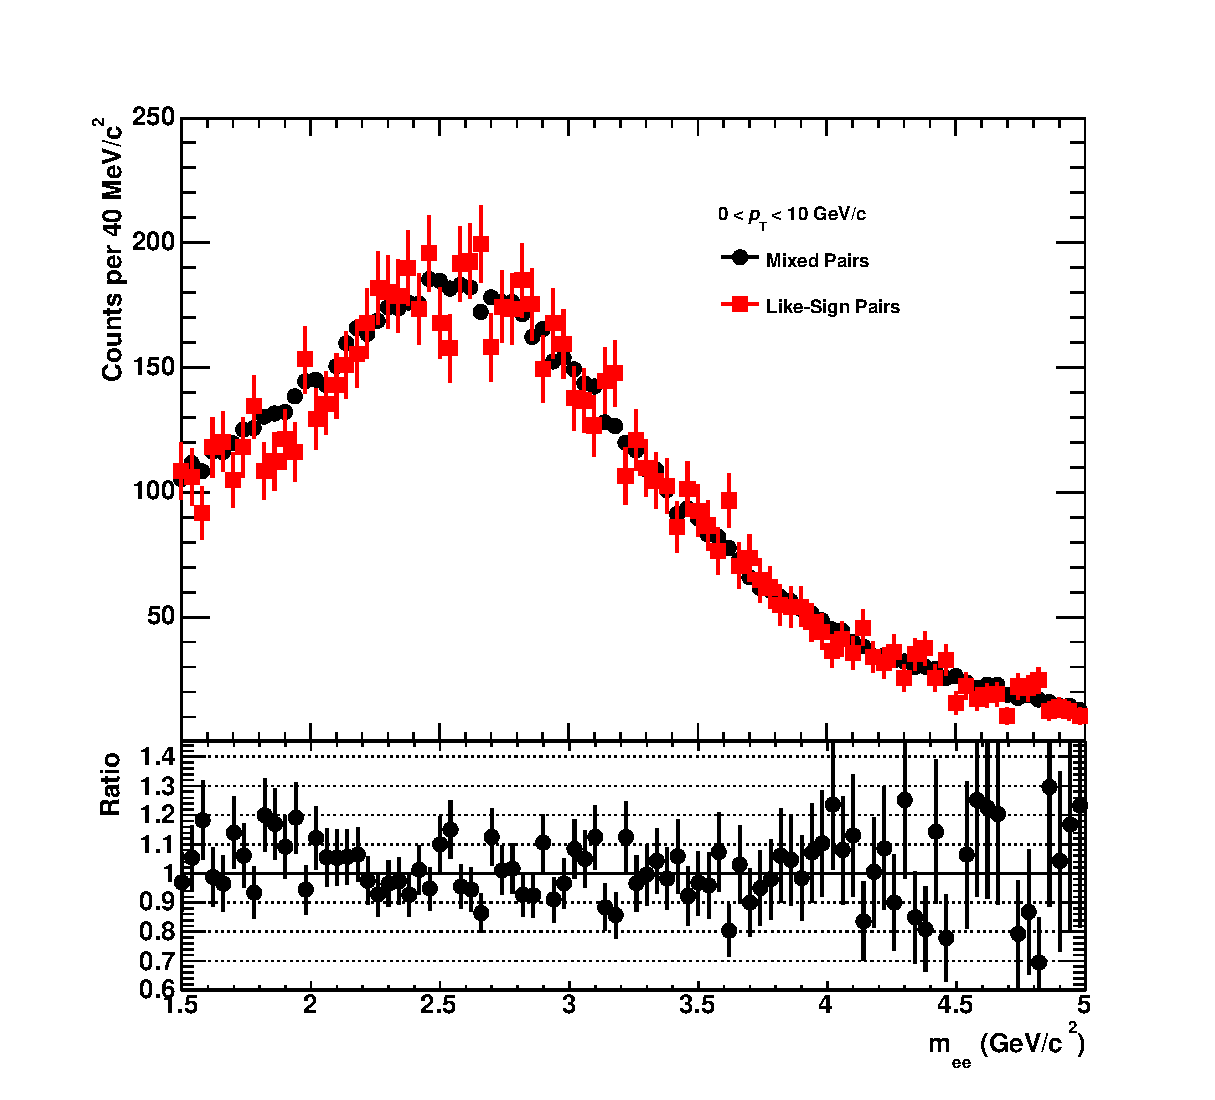
\includegraphics[width=10cm]{chap4/figure/SignalExtraction/BGComparison_MB.eps}
  \caption{Like-Sign background and event mixing pairs in p-Pb collisions (Upper) and the ratio of the number of entries between like-sign pairs and event mixing pairs. }
  \label{fig_4_bgcomp}
\end{figure}

%Significant difference between LS and Mixed background is not observed within the statistical uncertainty mainly from like-sign background. 
%Therefore the signal extraction is done by the event mixing technique and the residual background caused by mainly heavy flavor contributions is subtracted by the simultaneous fit of signal and background function.  
%The mixing pairs are not true shape of background. 
The main source of the systematic uncertainty of the background subtraction comes from the normalization and descripancy of true background shape. 
In oerder to evaluate the systematic uncertainty of background subtraction, following three methods are applied for the background subtraction. 

First, the mixing pairs are simply normalized by the yield in the side-band (2.0-2.5, 3.2-3.7 $GeV/c^{2}$). 
Raw $J/\psi$ yield is obtaned by subtracting the sclaed mixing pairs. 

Second method is a signal+background fitting. 
The signal shape is estimated from the full Monte-Calro calculation described in Section.~\ref{sec_4_correction}. 
The shape of the background is estimated by the event mixing. 
The fitting is performed with the fitting  range 2 $< ~m_{ee}~<$ 4 GeV$/c^{2}$.

In the third method, first of all the mixing pairs are scaled by the like-sign pairs and un-like sign pairs are subtracted by this sclaed mixing pairs. 
The subtracted yield contains mainly $J/\psi$ and correlated $c\bar{c}$.
The subtracted yield is fitted by the Signal function obtained by full Monte-Calro and the following exponential shape, 
\begin{equation}
  f(m_{ee}) = p_{0} e^{-(p_{1}m_{ee})^{p_{2}}}
\end{equation}
After the subtraction of the exponential component, raw $J/\psi$ signals are obtained. 
 

\subsection{Mass Shape of Reconstructed $J/\psi$}
The invariant mass shape of the measured $J/\psi$ signals is modified from the real mass shape of J/$\psi$ due to the following reasons, 
\begin{description}
  \item[-] Effects of the momentum resolution
  \item[-] Bremsstrahlung decay of electrons in the detectors. 
\end{description}
Therefore, the signal has long tail at the lower invariant mass side from the peak like Crystal-Ball function as shown Fig.~\ref{fig_4_jpsishape}.   
Figure~\ref{fig_4_jpsishape} shows the signal shape from MC and fitted Crystal-Ball function in some $J/\psi$ $p_{T}$ bins.
The mass shapes of reconstructed $J/\psi$ are described with Crystal-Ball functions and don't clear $p_{T}$ dependence. 
\begin{figure}[htbp]
 \begin{minipage}{0.5\hsize}
  \begin{center}
  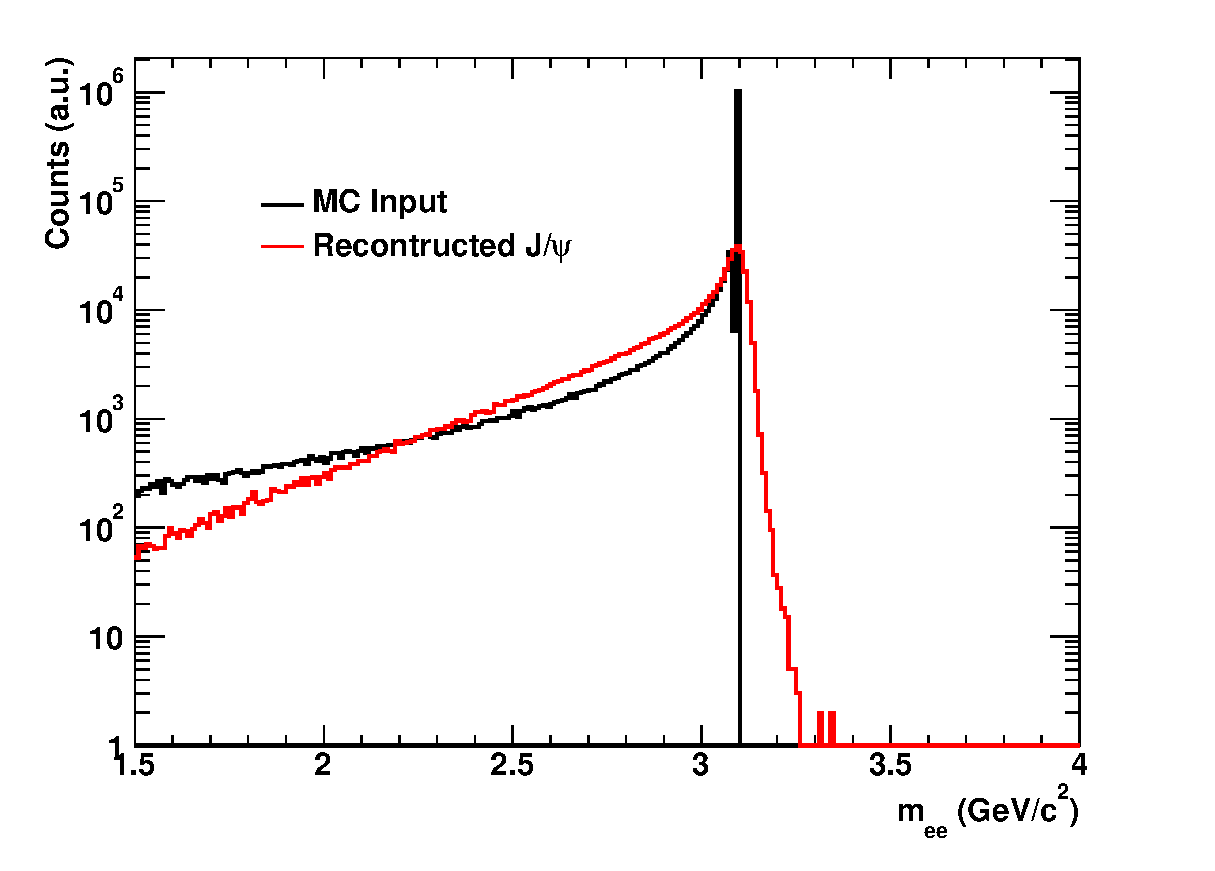
\includegraphics[width=8cm]{chap4/figure/SignalExtraction/MCInputandRecMassShape_LHC13d10.eps}}
  \end{center}
 \end{minipage}
 \begin{minipage}{0.5\hsize}
  \begin{center}
  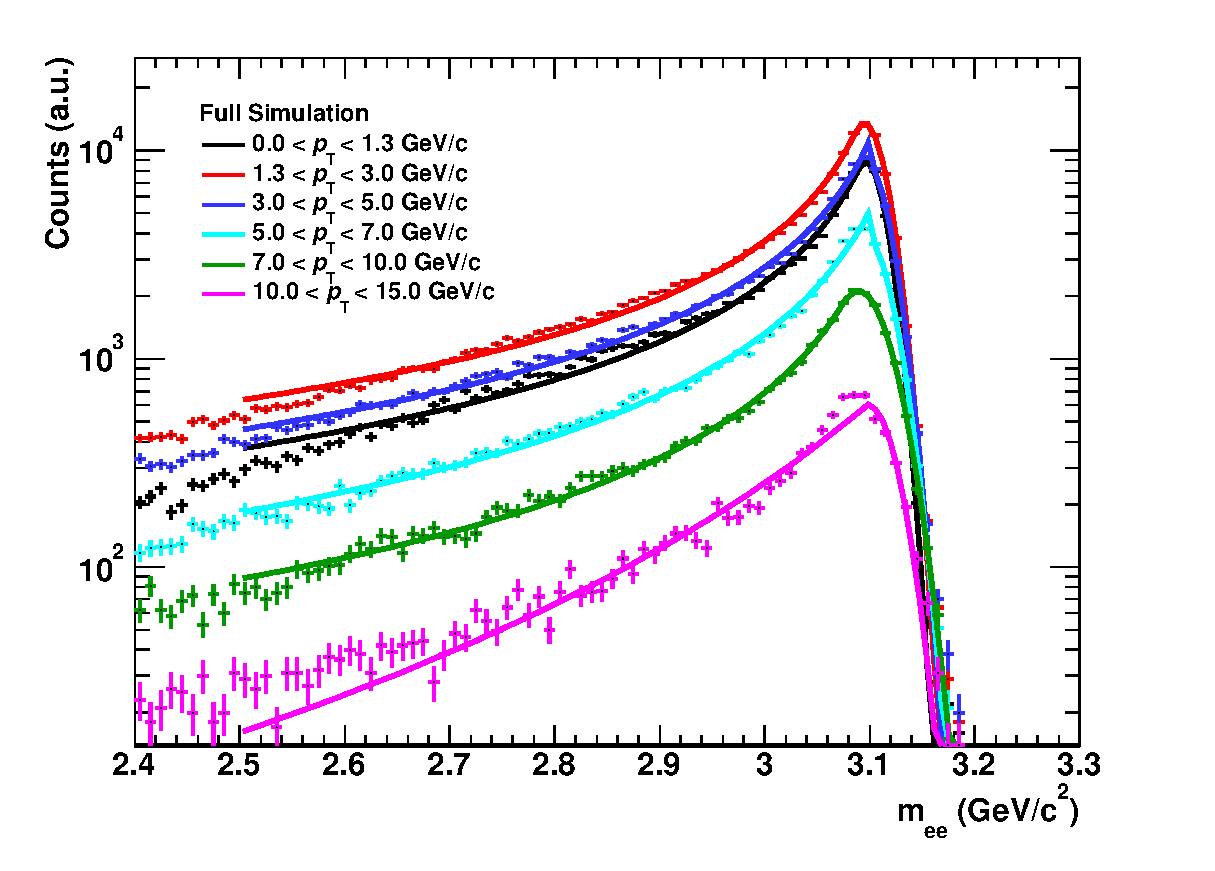
\includegraphics[width=8cm]{chap4/figure/SignalExtraction/MCRecontructedShape_LHC13d10.eps}
  \end{center}
 \end{minipage}
  \caption{Comparison of Reconstructed J/$\psi$ mass shape to the MC input mass (Left) and the $p_{T}$ dependence of estimated measured mass shape (Right). The solid curves show the Crystal-Ball fitting. }
  \label{fig_4_jpsishape}
\end{figure}

The left panel of Fig.~\ref{fig_4_jpsiuls} shows the invariant mass spectra of unlike sign pairs, and mixed events pairs, and the subtracted yield by the mixed pairs. 
Mixed pairs are normalized by the yield ratio to unlike-sign pairs at side-bands (2-2.5, 3.2-3.7 GeV/$c^{2}$).
%\begin{figure}[htbp]
% \begin{minipage}{0.5\hsize}
%  \begin{center}
%  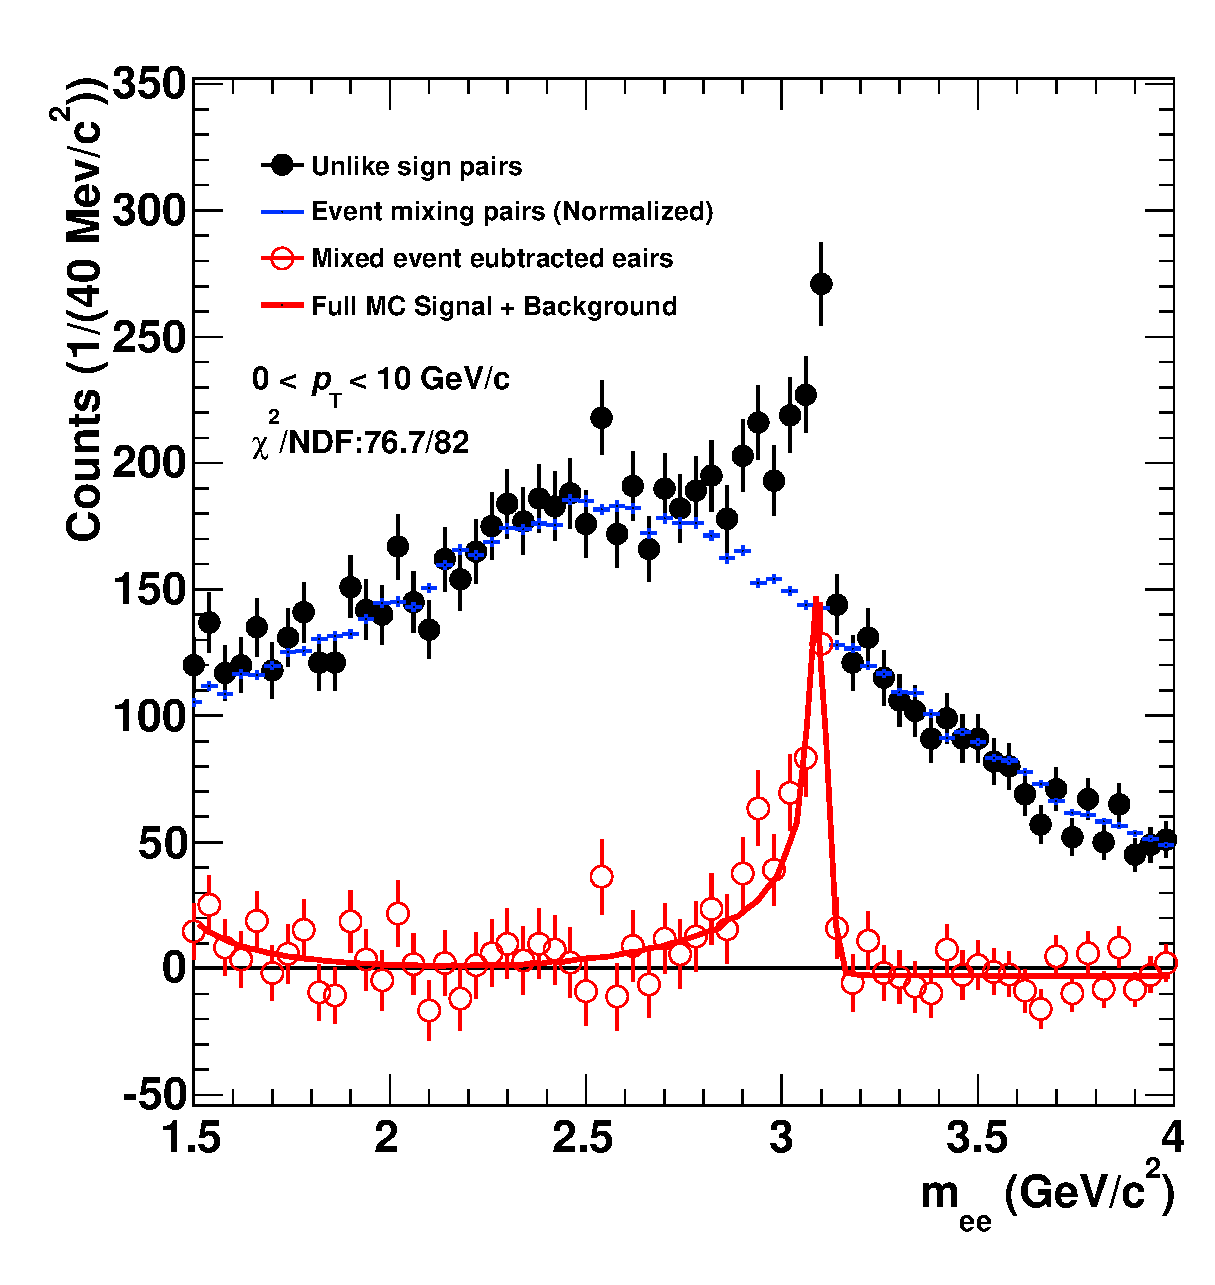
\includegraphics[width=8cm]{chap4/figure/RawYield/InclusiveULS_INT7_CutDetermination37.eps}}
%  \end{center}
% \end{minipage}
% \begin{minipage}{0.5\hsize}
%  \begin{center}
%  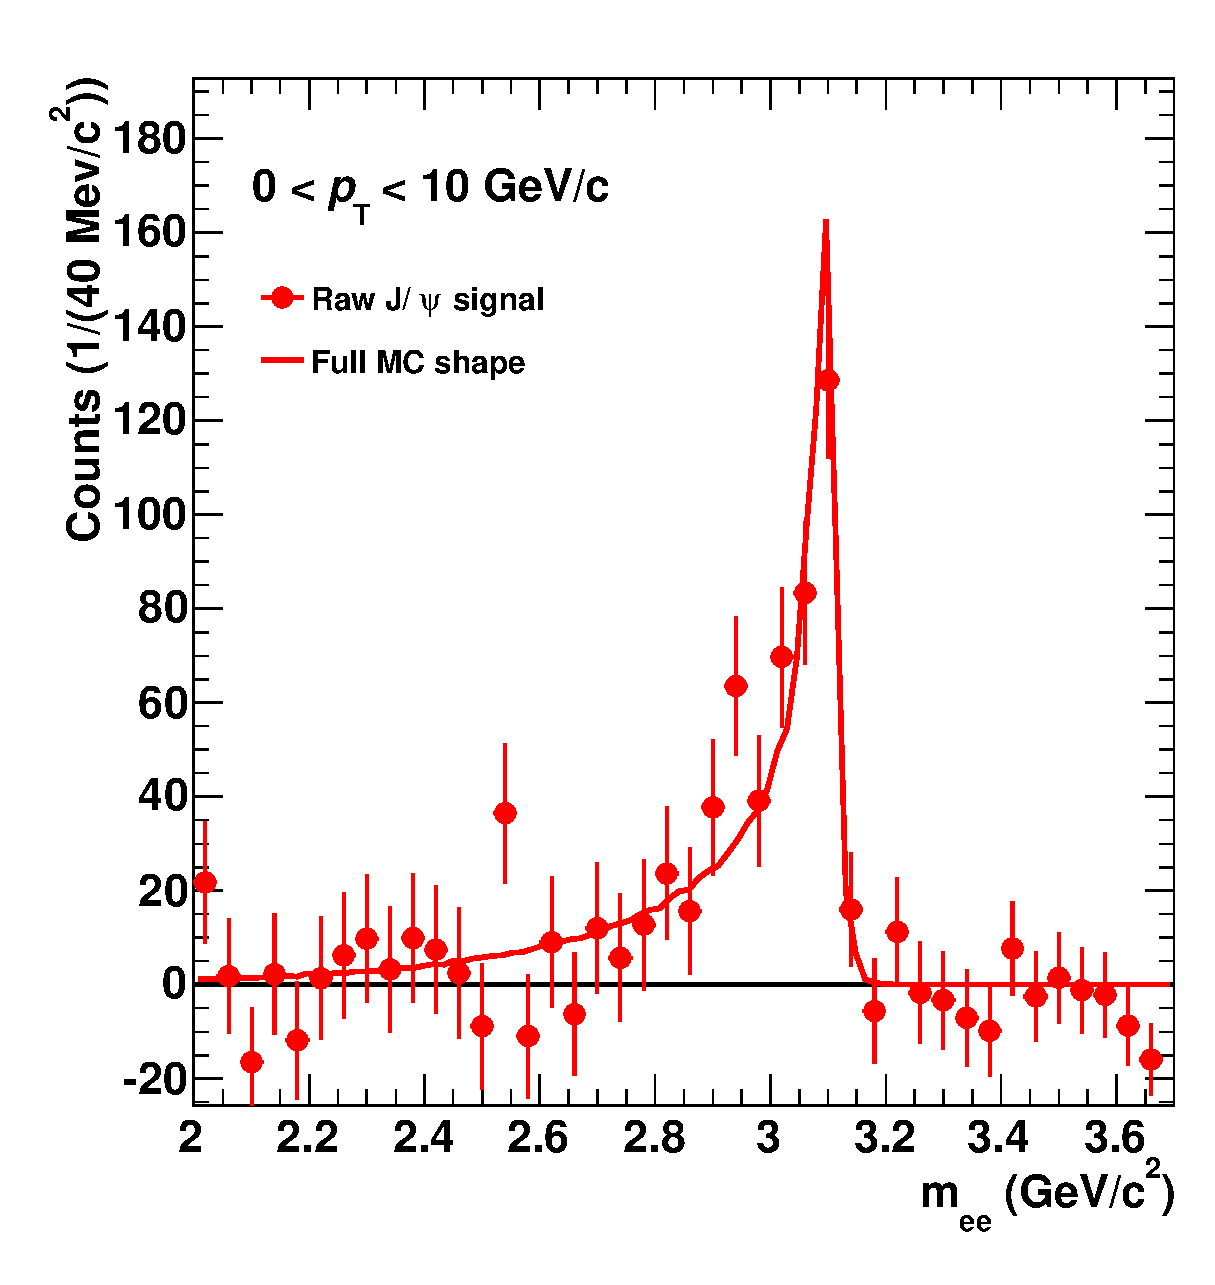
\includegraphics[width=8cm]{chap4/figure/RawYield/InclusiveRawYield_INT7_CutDetermination37.eps}
%  \end{center}
% \end{minipage}
%  \caption{ULS, Mixed background, and background subtracted yield (left) and $J/\psi$ raw signals and the fitting result by the shape of full Monte-Carlo simulation.}
%  \label{fig_4_jpsiuls}
%\end{figure}

After background subtraction by the event mixing, the subtracted pairs are fitted by the signal and background function. 
The function of the signals are taken from the histograms of the reconstructed $J/\psi$ in the full Monte-Carlo simulation. 
The background function is the $bg(m_{ee}) = \frac{a+bm_{ee}^{2}}{c+dm_{ee}+em_{ee}^{2}}$. 
The solid red curve of the left panel of Fig.~\ref{fig_4_jpsiuls} shows the result of fitting and the right panel of Fig.~\ref{fig_4_jpsiuls} shows the final raw signal of $J/\psi$. 
The fitting is done with good $\chi^{2}/NDF$. 
%\begin{equation}
 % bg(m_{ee}) = \frac{a+bm_{ee}^{2}}{c+dm_{ee}+em_{ee}^{2}}
%\end{equation}
%a, b, c, d, e are free parameters. 
%Finally the number of signal is extracted by bin counting within 2.92-3.16 GeV/$c^{2}$ after residual background subtraction. 
 
\subsection{Raw Signal Counting}
Since reconstructed mass shapes don't show the $\it{p}_{T}$ dependence, the same mass window of the signal counting is applied to all momentum bins and the number of raw signals is extracted by the bin-count method within the mass window. 

Figure~\ref{fig_4_masscutdep} show the mass window cut dependence of of signal to background and the significance. 
Signal to background increases with higher cutoff of the lower mass limit. 
On the other hand, the significance decreases above 2.94 due to the large lack of the signals as shown in Fig~\ref{fig_4_masscuteff}. 

Therefore, the number of signals are counted as the sum of the bin contents within 2.92 - 3.16 GeV/$c^{2}$ with 70\% efficiency.
\begin{figure}[htbp]
 \begin{minipage}{0.5\hsize}
  \begin{center}
  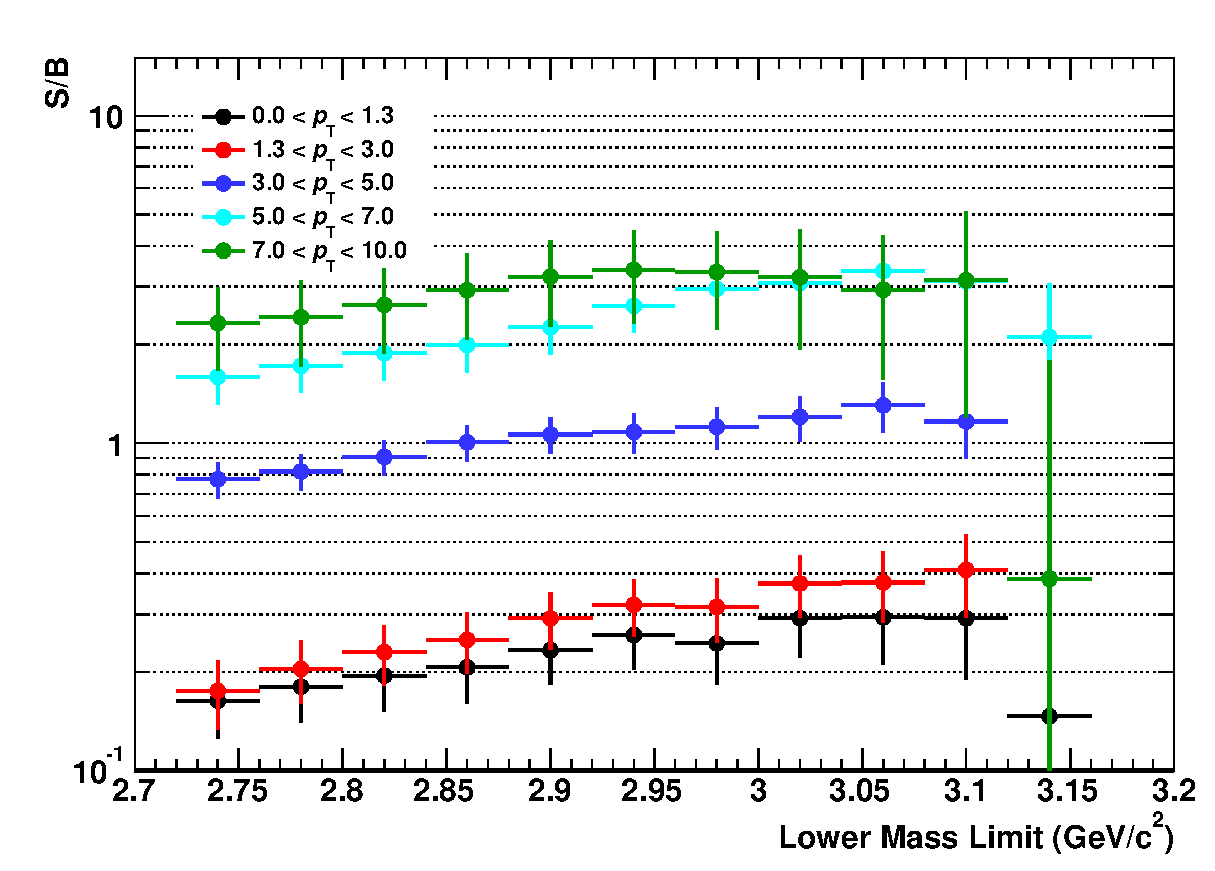
\includegraphics[width=8cm]{chap4/figure/SignalExtraction/MassCutDep_SB_MB.eps}}
  \end{center}
 \end{minipage}
 \begin{minipage}{0.5\hsize}
  \begin{center}
  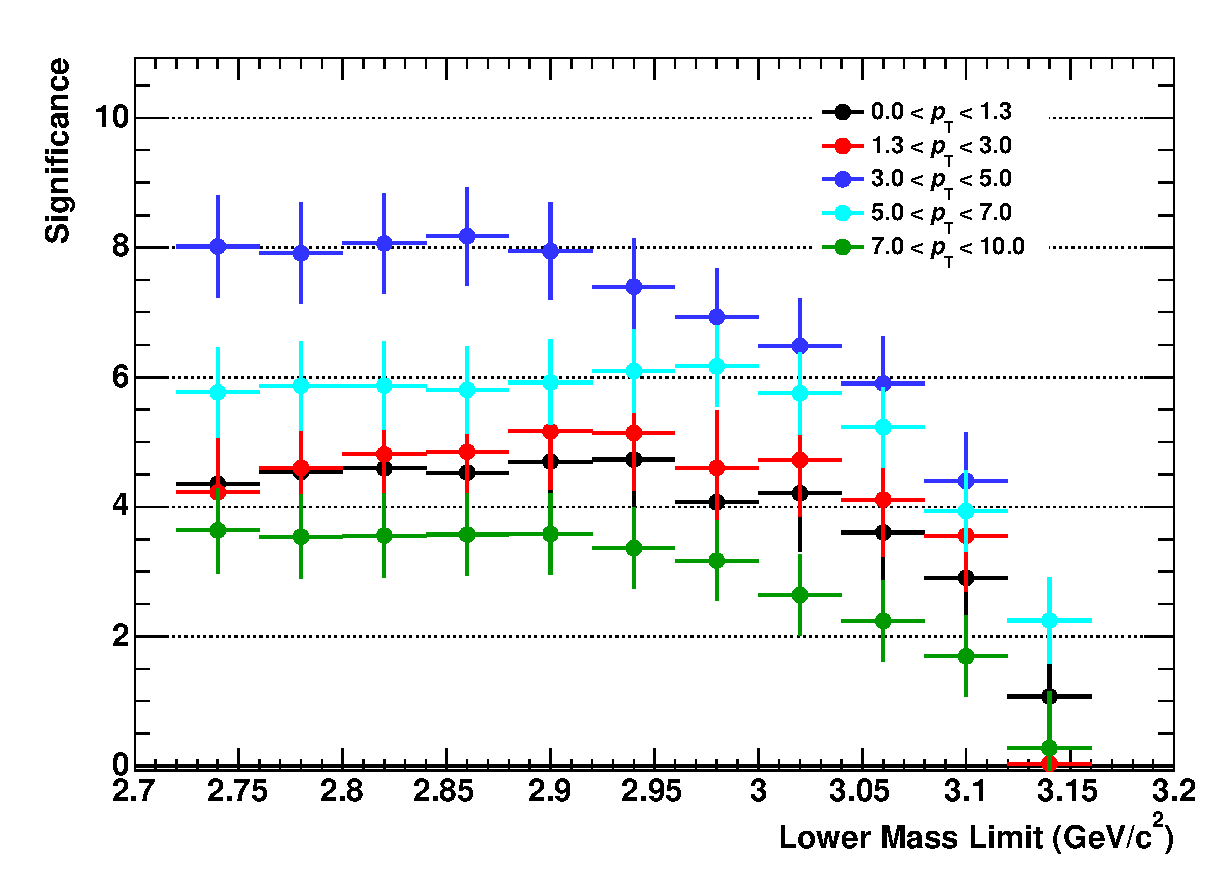
\includegraphics[width=8cm]{chap4/figure/SignalExtraction/MassCutDep_Significance_MB.eps}
  \end{center}
 \end{minipage}
  \caption{Mass window cut dependence of the signal to background and the significance of $J/\psi$ signals.}
  \label{fig_4_masscutdep}
\end{figure}

\begin{figure}[!h]
  \centering
  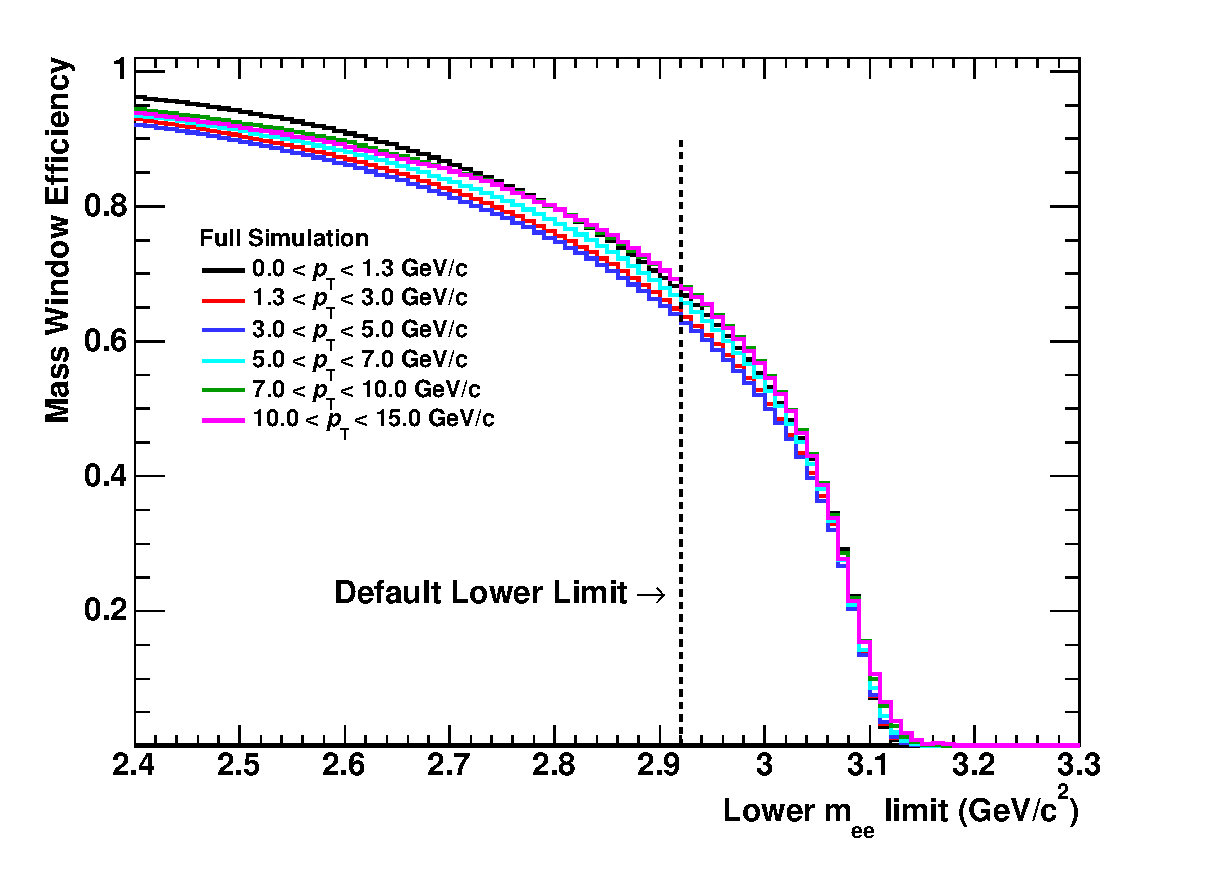
\includegraphics[width=8cm]{chap4/figure/SignalExtraction/JpsiRawYieldMassWindowCutDep.eps}
  \caption{Invariant mass window efficiency as a function of lower mass limit. }
  \label{fig_4_masscuteff}
\end{figure}


\subsection{Summary of Cut Parameters and Raw Signals}
The main parameters to be optimized are SPD hit requirement and TPC electron identification cuts. 
72 combinations of cut parameters are checked and the final cut setting is determined to maximize the significance. 
Qualitatively, the cut setting of lower $p_{T}$ bins are tuned to increase the signal to background ratio. 
On the other hand, at higher $p_{T}$ bins, the parameters are optimized to maximize the number of signals. 
\begin{table}[!h]
  \centering
    \begin{tabular}{ccccc} \hline
      $p_{T}$ bin (GeV/c)  & $p^{e}_{T}$ cutoff (GeV/c) & SPD hit & TPC n$\sigma_{pion}$ & TPC $\sigma_{proton}$\\ \hline
      0-10          & 1.0   & First     &     3.0                          & 3.5                                      \\ 
      0-1.3         & 1.0  & First   &     3.0                           & 3.5                                      \\ 
      1.3-3         & 1.0  & First   &     3.5                          & 3.5                                      \\ 
      3-5           & 0.8  & Any     &     3.0                           & 3.5                                      \\ 
      5-7           & 1.0  & Any     &     3.0                           & 3.5                                      \\ 
      7-10          & 1.0  & Any     &     3.0                           & 3.0                                      \\  \hline
    \end{tabular}
\caption{Summary of the cut parameters.}
\end{table}
  \begin{table}[!h]
  \centering
  \begin{tabular}{ccccc} \hline
    $p_{T}$ bin (GeV/c) & Raw Yield & Signal/Background & Significance & $\chi^{2}/NDF$ \\ \hline
     0-10               &           &                    &              & \\
      0-1.3             &           &                    &              & \\
      3-5         &&&& \\
      5-7          &&&& \\
      7-10          &&&& \\  \hline
 \end{tabular}
  \caption{Summary the number of reconstructed $J/\psi$, signal to background ratio, significance, and $\chi^2/NDF$ of the signal fitting.}
\end{table}

%For the crosscheck of signal extraction, direct Signal+Background fitting was checked. 

\section{Acceptance and Efficiency Correction}

\section{Monte-Carlo Simulation}
\label{sec_4_mc}
The acceptance and reconstruction efficiency is evaluated  using Monte-Calro simulation.  
In this analysis, the following Monte-Carlo productions are used,  
\begin{itemize}
\item[-] p-Pb minimum bias production with DPMJet~\cite{bib_dpmjet} 
\item[-] Single $J/\psi$ and the minimum biass Hijing p-Pb mixture production~\cite{bib_hijing}
\end{itemize}
The input single of enhanced $J/\psi$ spectrum is weighted according to the pp reference described in Section~\ref{sec_4_ppref}.
$J/\psi$ is forced to decay into dielectron channels including the radiative decay ($J/\psi\rightarrow \gamma e^{+}e^{-}$) with the decay table of Pythia~\cite{bib_pythia}. 

Both productions are full Monte-Carlo productions which include the track reconstruction and material effects in the ALICE detectors calculated by the GEANT3 simulation~\cite{bib_geant}.  
The all parameters of the detector calibration are anchored by the run condition and the statistical weighting for each run is also applied to avoid the discrepancy to the real data set. 

The latter $J/\psi$ enhance production is used for the signal extraction and efficiency calculation.
DPMJet production is used to evaluate the performance of track quarlity and electron identification with the conversion electrons.

\label{sec_4_correction}
The detection efficiency including the geometrical acceptance is evaluated with the following definition, 
\begin{equation}
  Acce\times \epsilon = \frac{\rm{The~ number~ of~ reconstructed}~ J/\psi ~\rm{in}~ |y| < 0.9}{\rm{The~number~of~generated}~J/\psi ~in~ |y| < 0.9}
\end{equation}
Figure~\ref{fig_4_jpsieff_pt}, \ref{fig_4_jpsieff_y} show the step-by-step $J/\psi$ efficiency as a function of $p_{T}$ and $y$.
Over all efficiency is 10\%-20\% in all $p_{T}$ region. 
%\subsection{Single Electron Efficiency}
%\subsection{Pair Correction}
\begin{figure}[!h]
  \centering
  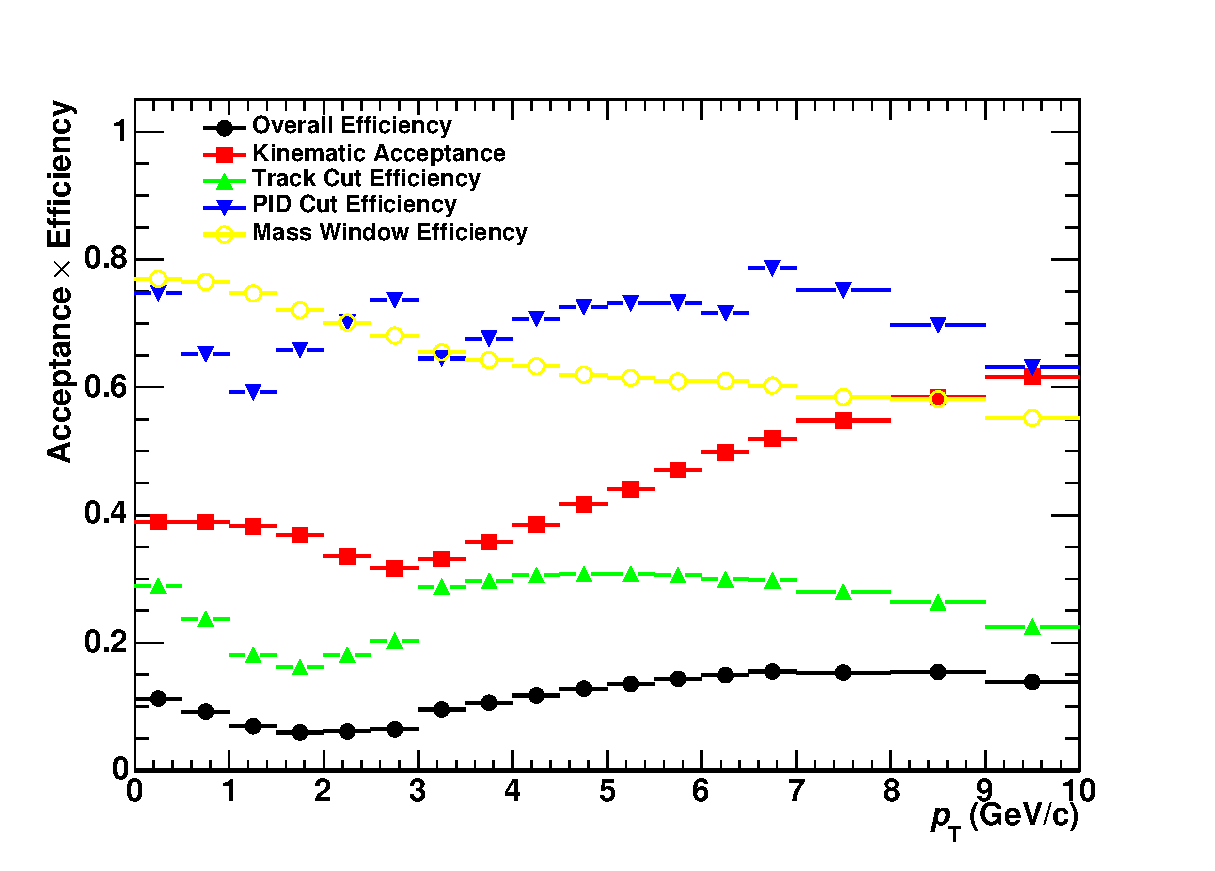
\includegraphics[width=10cm]{chap4/figure/Correction/JpsiEff_pt_stepbystep.eps}
  \caption{Step-by-step acceptance $\times$ efficiency of $J/\psi$ as a function of $p_{T}$.}
  \label{fig_4_jpsieff_pt}
\end{figure}

\begin{figure}[!h]
  \centering
  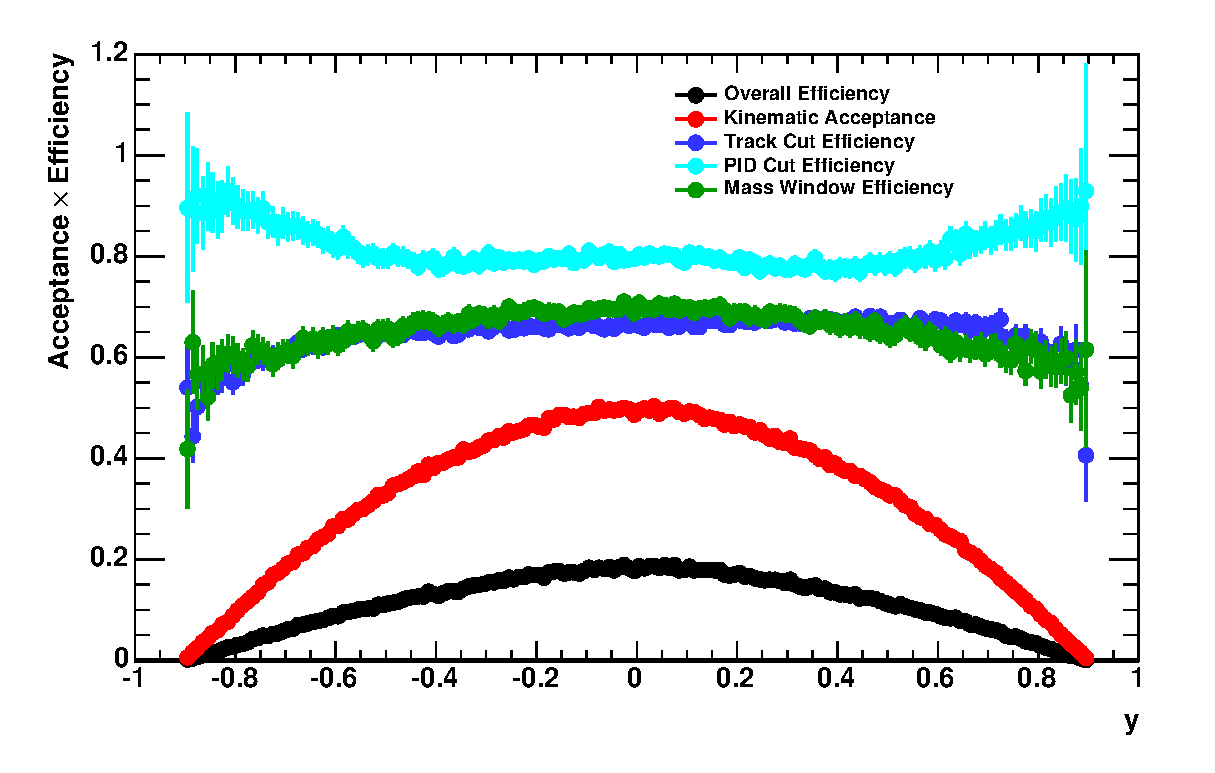
\includegraphics[width=10cm]{chap4/figure/Correction/JpsiEff_y_stepbystep.eps}
  \caption{Step-by-step acceptance $\times$ efficiency $J/\psi$ as a function of y.}
  \label{fig_4_jpsieff_y}
\end{figure}

Due to the detector effects, the reconstructed $p_{T}$ is not same as the true $p_{T}$. 
Therefore the additional correction is needed to extract the invariant spectrum if it causes the serious modification. 
If the input spectrum is reasonable to the true $J/\psi$, this correction can be done by taking the ratio of reconstructed $p_{\rm{T}}$ spectrum to true $p_{\rm{T}}$ spectrum in Monte-Carlo simulation.
Figure\ref{fig_4_jpsieff_cutdep} shows the comparison of reconstructed $p_{T}$ spectra and true $p_{T}$ spectra. 
The large discrepancy between reconstructed $p_{T}$ and true $p_{T}$ is observed without invariant mass selection. 
With the invariant mass selection, the signals within the strict kinematic selection are already selected and the ratio is consistent with unit.
The ratio of reconstructed $p_{T}$ and true $p_{T}$ is taken as the correction for each momentum bin.  
\begin{figure}[!h]
  \centering
  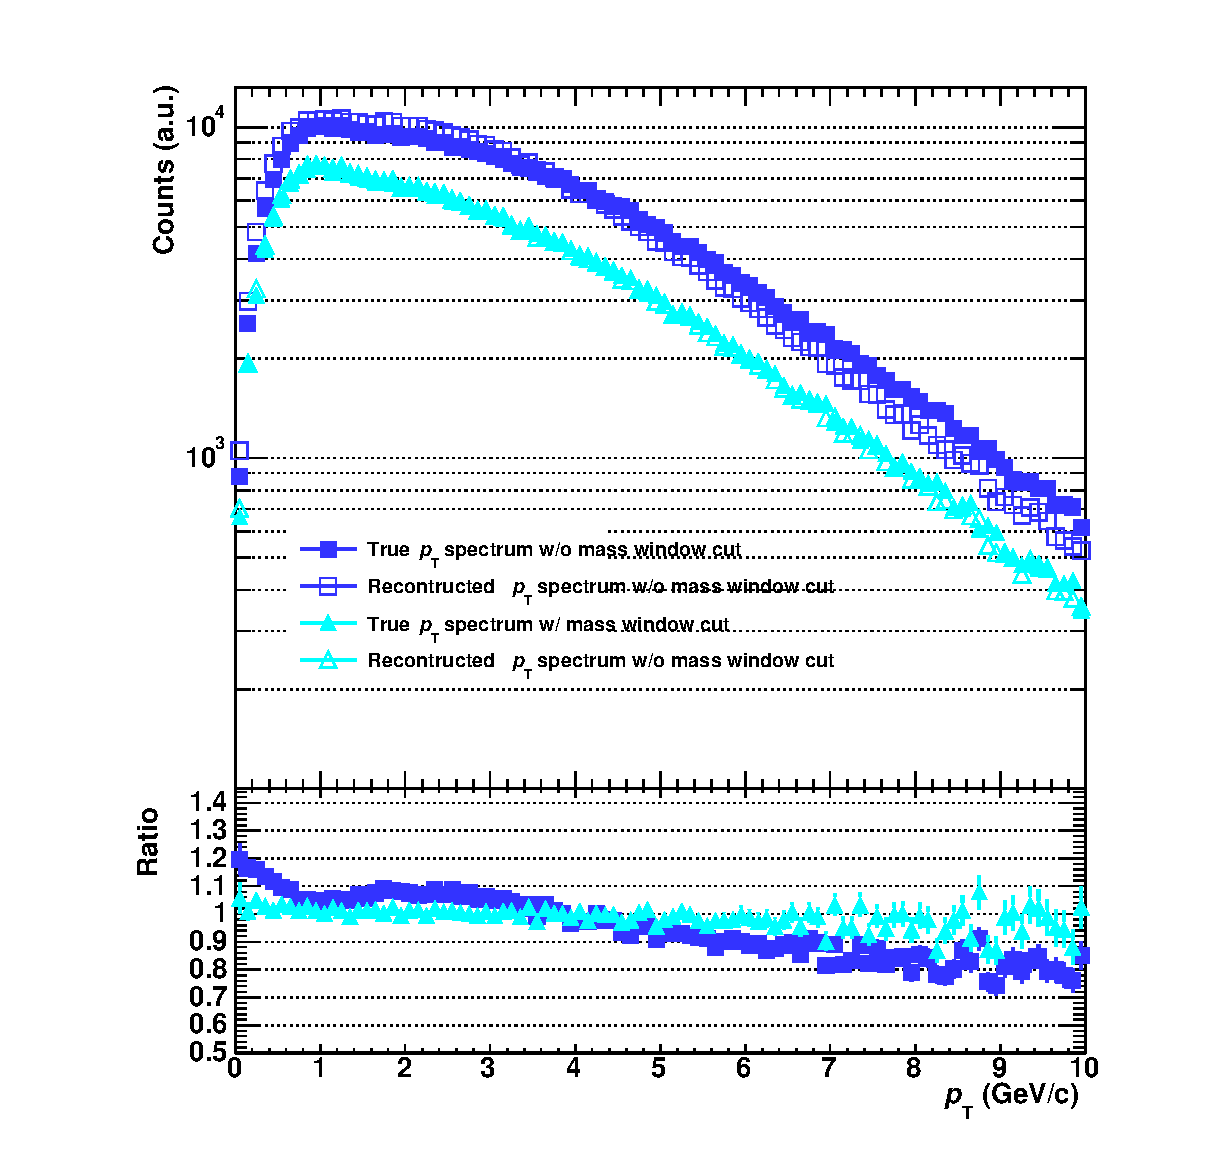
\includegraphics[width=10cm]{chap4/figure/Correction/JpsiRecPtSpectra.eps}
  \caption{Comparison of the reconstructed $p_{T}$ and true $p_{T}$ spectra (Upper) and their ratio (Lower). The blue markers and the cyan markers show the spectra without mass window cut and with mass window cut requirement, respectively. The closed markers express the reconstructed $p_{T}$ spectra and the open markers show the true $p_{T}$ spectra.}
  \label{fig_4_jpsieff_cutdep}
\end{figure}

The input $p_{T}$ spectrum of $J/\psi$ affected on the efficiency evaluation in the wide bins. 
Basically the input spectrum is produced by the pp reference. 
%However it doesn't give a complete description of the true input spectrum. 
The efficiency calculation is performed with this $p_{T}$ weighting first. 
After the first correction, the corrected spectrum is fitted with the following function. 
\begin{equation}
  f(p_{T}) = C_{1}\frac{p_{T}}{\light( 1+ (\frac{p_{T}}{C_{0}}^{2})^{C_{2}})}
\end{equation}
The efficiency is calculated again with the above fitting function and the final corrected yield is extracted. 
The RMS of the first and second efficiency values is taken as the systematic errors. 


%\section{Trigger Efficiency Correction}
%In this analysis, the trigger efficiency is defined by
%\begin{equation}
%Trigger Efficiency = \frac{The number of triggered track for the all reconstructed tracks in the offline }{The number of all reconstructed tracks in the offline tracking}
%\end{equation}
%For the evaluation

%\subsection{Single Electron Efficiency}

%figure of single electron efficiency as a function of pt
%figure of single electron spectra

%\subsection{Pair Correction}
%Pair trigger efficiency can be  defined as following, 
%\begin{equation}
 % \epsilon^{Trig} _{pair}
%\end{equation}

\section{Systematic Uncertainty Evaluation}
\label{sec_4_syst}
\subsection{Track Reconstruction and Electron Identification}
The following cut variation is applied to extract the systematic uncertainty on the track quality cuts. 
\begin{description}
  \item[-] The number of TPC clusters: 60, 70 (default),  80, 100.
  \item[-] TPC $\chi^{2}$ per the number of clusters: 3.5, 4 (default), 4.5.
\end{description}
In order to reduce the statistical fluctuation, this systematic uncertainty evaluation is done for the $p_{T}$-integrated yield since the detector performance doesn't depend on $p_{T}$ strongly as described in Section\ref{sec_4_trackrec}. 
The RMS of these variation is taken as the systematic uncertainty. 
For electron identification, the following variation is considered and RMS of these variation is caclculated as the systematic uncertainty.
\begin{description}
  \item[-] TPC inclusion cut: 2, 3, 3.5. 
  \item[-] TPC Pion exclusion cut: default cut value $\pm$ 0.5. 
  \item[-] TPC proton exclusion cut: default cut value $\pm$ 0.5.
\end{description}

\subsection{Signal Extraction}
%\subsubsection{Background Subtraction}
The raw number of signals are counted by the integration of the bin contents within the mass window. 
In order to estimate this systematic uncertainty, the integrated value of the signal fitting function is considered. 
As the reference of $J/\psi$ signals, the reconstructed $J/\psi$ shape from the full Monte-Carlo production is used. 
The reference of $J/\psi$ shape can be obtained from the reconstruction efficiency of single electrons. 
The RMS of these methods are taken as the systematic uncertainty. 

\subsubsection{Mass Window Cut}
Figure~\ref{fig_4_symassdep} shows the $p_{T}$ dependence of reconstructed $J/\psi$ mass shapes in the Monte-Carlo simulation. 
At lowest 2 bins shows the same trends and highest 2 bins also show the similar trend. 
Therefore they are merged to reduce the statistic fluctuation for the systematic uncertainty estimation of the mass window selection.  
The following cut variation is applied and RMS of all combination is taken as the systematic uncertainty. 
\begin{description}
  \item[-] Lower limit: 2.84, 2.92 (default) , 3.0 (GeV/$c^{2}$).
  \item[-] Higher limit: 3.12, 3.16 (default), 3.2 (GeV/$c^{2}$) .
\end{description}
\begin{figure}[!h]
  \centering
  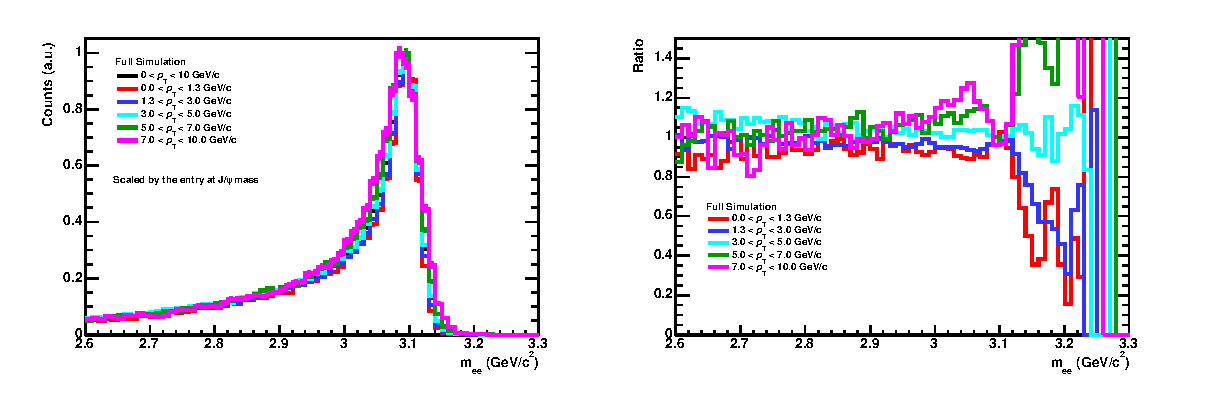
\includegraphics[width=15cm]{chap4/figure/Systematics/MCRecontShape_PtDep_LHC13d10.eps}
  \caption{ }
  \label{fig_4_symassdep}
\end{figure}


\subsection{Monte-Carlo weighting}
As described in Section~\ref{sec_4_correction}, two $p_{T}$ weighting functions are checked for the efficiency evaluation. 
%By default, the input $p_{T}$ spectrum is taken as the pp spectra described in Section~\ref{sec_4_ppref}. 
The RMS of efficiency variation with these input spectra is taken as the systematic uncertainty of the input $p_{T}$ spectrum.  
%The other spectrum estimated weighted by the modified hagedron spectrum obtained from charged particle spectrum in p-Pb is also checked. 


\subsection{Normalization factors}
The following uncertainties are considered to extract the cross section and $R_{pPb}$. 
\begin{description}
  \item[-] $\sigma_{V0}$: 2.09 $\pm$ 0.06 b~\cite{bib_v0cross}.
  \item[-] Branching Ratio of J/$\psi\rightarrow e^{+}e^{-}$: 5.94 $\pm$ 0.06 \% ~\cite{bib_pdg}.
  \item[-] $T_{pPb}$: 0.0983 $\pm$ 0.0035 $mb^{-1}$ ~\cite{bib_tppb}.
\end{description}


\subsection{Summary of Systematic Uncertainty}
Figure~\ref{fig_4_syssummary} shows the summary of the relative systematic uncertainties as a function of $p_{T}$. 
%The $p_{T}$ integrated results is summarized. 

\begin{figure}[!h]
  \centering
  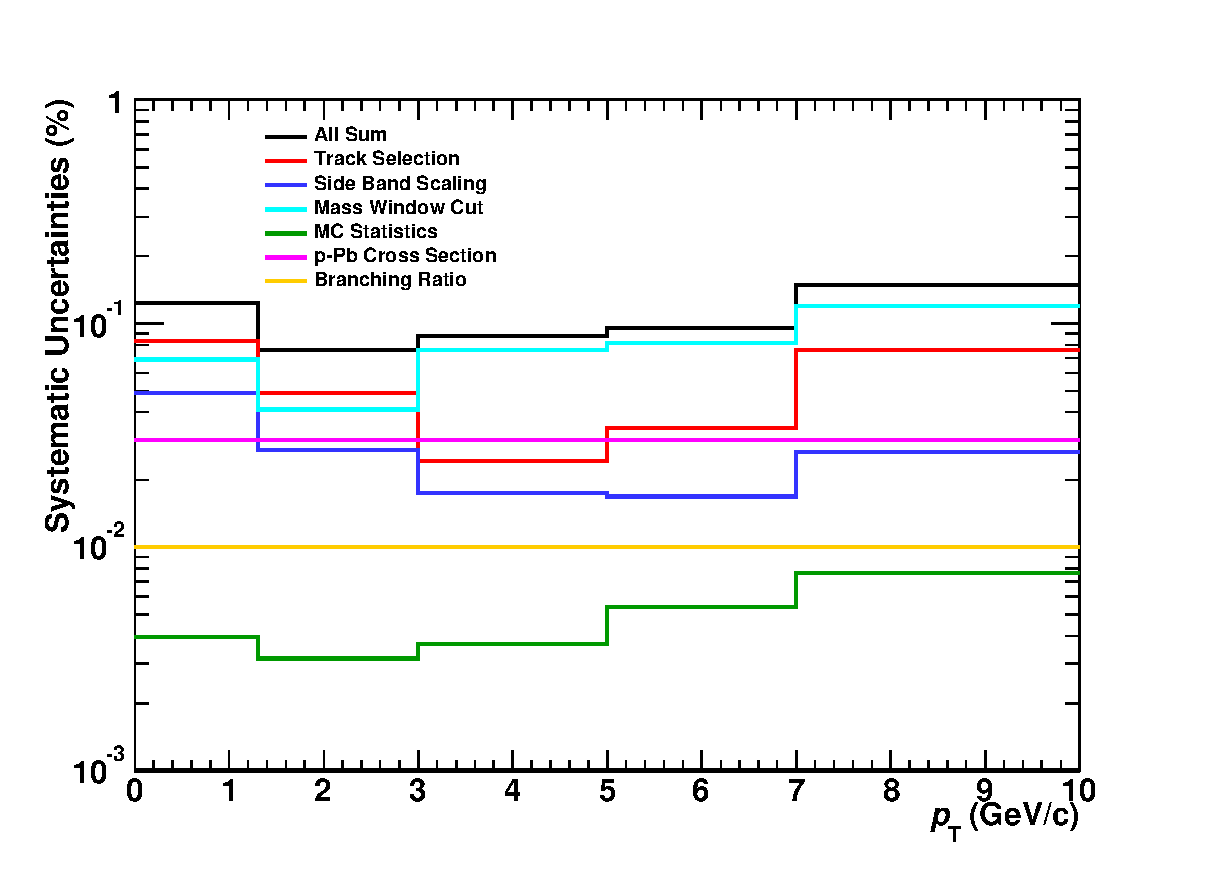
\includegraphics[width=10cm]{chap4/figure/Systematics/JpsiSys_INT7_ptdep.eps}
  \caption{Summary of the relative systematic uncertainties.  }
  \label{fig_4_syssummary}
\end{figure}

\section{Extraction of the pp Reference spectra}
\label{sec_4_ppref}
It is very important to compare the results with pp reference data for the study of cold nuclear matter effects. 
However, unfortunately, there is no results of the pp collisions at $\sqrt{s_{NN}} =$5.02 TeV.
The procedure of the interpolating in this analysis refer to~\cite{bib_jpsippref}.
The reference spectra is interpolated phenomenologically from the measured cross section in pp at RHIC, Tevatron, and LHC.
We briefly explain how to extract the pp reference spectrum in this section. 
The inclusive $J/\psi$ cross section at mid-rapidity is extracted by functional fitting approach and theoretical model comparison. 
The value is
\begin{equation}
  BR(J/\psi\rightarrow ee)~\times ~d\sigma/dy_{y\sim0, \sqrt{s}=5.02TeV}~=~367.8~\pm~9.9\%~(stat)~\pm~ 13.3\% ~(syst) ~\rm{nb}
\end{equation}  
The rapidity dependence is negligible compared to other uncertainties. 
The transverse momentum dependence is extended as following. 
First, the  double differential cross section $d^{2}\sigma/dp_{T}dy$ was normalized by the $p_{T}$-integrated cross section to unity. 
Then the transformation of $p_{T} \rightarrow p_{T}/<p_{T}>$ is done in order to approach the universal behavior. 
In this study the statistical and systematic uncertainties for all observables have been summed in quadrature.
The $\sqrt{s}$ dependency of $\langle p_{T}\rangle$ is calculated by fitting with several functions. 
The scaled spectra can be fitted with the following function, 
\begin{equation}
  \frac{\langle p_{T}\rangle}{d\sigma/dy}\frac{d^{2}\sigma}{dp_{T}dy} = \frac{2(n-1)B^{2}p_{T}/\langle p_{T}\rangle }{(1+B^{2}(p_{T}/\langle p_{T}\rangle)^{2})^{n}}
\end{equation}
where B is $\Gamma(3/2)\Gamma(n-3/2)/\Gamma(n-1)$. 
n is determined as 3.79 $\pm$ 0.07 with $\chi^{2}/ndf=$ 0.6.
Figure~\ref{fig_4_ppfit} show the result of the scaled fitting. 
The determination of the systematic uncertainty on the fit procedure was evaluated by performing several fits to the data and excluding one by one the experimental results for a given energy. 
The main contribution to the systematic uncertainty came from the residual $\sqrt{s}$ dependence.

The interporated values are summarized in Table.~\ref{table_4_pprefvalue}.
The both of the statistical and the systematic uncertainties are propagated as a systematic uncertainty of pp reference. 

If the uncertainty of $J/\psi$ cross section is fully correlated. 
The un-correlated uncertainty is determined by the interporated spectra calculated with various setting of $\langle p_{T}\rangle$ and n. 
The mean points of $p_{T}$ differential pp reference are calculated with $\langle p_{\rm{T}}\rangle=$2.771 GeV/c and n=3.79. 
The deviation is calculated by the different setting as shown in Fig.~\ref{fig_4_ppref} and theier RMS of these valiation is used for systematic unceratainty evaluation. 
%The difference from the meanp point is taken as the un-correlated systematic unceratainty. 
Figure~\ref{fig_4_ppref} shows the interpolated pp reference $J/\psi$ spectrum in pp at $\sqrt{s_{NN}}=$5.02 TeV and comparison to the measured spectra at different energies. 
The band of the spectra include both of correlated and uncorrelated uncertainties. 
\begin{table}
  \centering
  \begin{tabular}{ccc} \hline
    Rapidity   & $d\sigma/dy (\mu b)$  & $\langle p_{T} \rangle$ \\ \hline
    $|y|<$0.9  & 6.192$\pm$0.613$\pm$0.824  & 2.771$\pm$0.095$\pm$0.106 \\
    2.5$<y<$4  & 5.272$\pm$0.363$\pm$0.105  & 2.424$\pm$0.029$\pm$0.024 \\ \hline
  \end{tabular}
  \caption{Interporated $d\sigma/dy$ and $\langle p_{T}\rangle$ in pp collisions at $\sqrt{s}=$5.02 TeV.}
  \label{table_4_pprefvalue}
\end{table}


\begin{figure}[!h]
  \centering
  \includegraphics[width=15cm]{chap4/figure/ppref/scalefit.png}
  \caption{Scaled fit (left) and Ratio (right) to the experimental results to several measured spectra in PHENIX, CDF, MCS, LHCb, and ALICE~\cite{bib_jpsippref}. 
  }
  \label{fig_4_ppfit}
\end{figure}


\begin{figure}[!h]
  \centering
  \includegraphics[width=10cm]{chap4/figure/ppref/ppref5TeV_uncorrsys.eps}
  \caption{Systematic study of $\langle \it{p}_{T}\rangle$ and n variation dependence of interporated pp reference spectrum at $\sqrt{s}=$5.02 TeV.. }
  \label{fig_4_ppref}
\end{figure}

\begin{figure}[!h]
  \centering
  \includegraphics[width=10cm]{chap4/figure/ppref/ppspectra.png}
  \caption{Experimental and interpolated spectra in pp collisions~\cite{bib_jpsippref}.}
  \label{fig_4_ppref}
\end{figure}


